\documentclass[tikz,border=0pt]{standalone}
\usepackage{xcolor}
\usetikzlibrary{calc}
% Palette: Sam_Comm_final.png by eye, each course's own, and data/frogs.json.
\definecolor{ink}{HTML}{3B2340}
\definecolor{sky}{HTML}{EFC46A}
\definecolor{skyhi}{HTML}{F5DA92}
\definecolor{skylow}{HTML}{E9B060}
\definecolor{cloud}{HTML}{F2D58A}
\definecolor{paper}{HTML}{FBEFD0}
\definecolor{cream}{HTML}{FFF6E0}
\definecolor{white}{HTML}{FFFFFF}
\definecolor{wallA}{HTML}{E88A73}
\definecolor{wallB}{HTML}{EE9F7E}
\definecolor{wallC}{HTML}{E47A7E}
\definecolor{wallD}{HTML}{F0B07E}
\definecolor{wallE}{HTML}{D9765F}
\definecolor{wallF}{HTML}{E99A8A}
\definecolor{greenA}{HTML}{8DBB7E}
\definecolor{greenB}{HTML}{6FA77A}
\definecolor{greenC}{HTML}{A9C97F}
\definecolor{greenD}{HTML}{5E9C6A}
\definecolor{greenE}{HTML}{4A8060}
\definecolor{meadow}{HTML}{B5CF86}
\definecolor{meadowdark}{HTML}{9DBE74}
\definecolor{window}{HTML}{F6E7A0}
\definecolor{windark}{HTML}{8C5A64}
\definecolor{metal}{HTML}{8D9A93}
\definecolor{metaldark}{HTML}{5E6B66}
\definecolor{wood}{HTML}{B9835A}
\definecolor{wooddark}{HTML}{8C5A3C}
\definecolor{woodlight}{HTML}{D9A66F}
\definecolor{rope}{HTML}{E3C48A}
\definecolor{stone}{HTML}{E7C9A0}
\definecolor{stonedark}{HTML}{C9A47E}
\definecolor{road}{HTML}{8E7A86}
\definecolor{roadline}{HTML}{F6E7A0}
\definecolor{kerb}{HTML}{D8B48C}
\definecolor{red}{HTML}{E0483E}
\definecolor{redlight}{HTML}{F27A6A}
\definecolor{gold}{HTML}{FFB000}
\definecolor{goldlight}{HTML}{FFD54F}
\definecolor{bell}{HTML}{F2B53A}
\definecolor{teal}{HTML}{4FA3A0}
\definecolor{tealdark}{HTML}{3C8582}
\definecolor{magenta}{HTML}{FF2E88}
\definecolor{cyan}{HTML}{13CFE3}
\definecolor{violet}{HTML}{8A5BD6}
\definecolor{water}{HTML}{6FB3A8}
\definecolor{waterlight}{HTML}{9FD3C6}
\definecolor{waterdark}{HTML}{4F8E86}
\definecolor{pad}{HTML}{7DB86A}
\definecolor{paddark}{HTML}{5C9A52}
\definecolor{padlight}{HTML}{A6D38A}
\definecolor{reed}{HTML}{8DB26A}
\definecolor{cattail}{HTML}{8A5A3C}
\definecolor{moss}{HTML}{A8B88E}
\definecolor{cypress}{HTML}{5E8A5A}
\definecolor{cypressdark}{HTML}{4A7048}
\definecolor{lotus}{HTML}{F48FB1}
\definecolor{lotusdark}{HTML}{E06C98}
\definecolor{lotuslight}{HTML}{FAD0DF}
\definecolor{lotuscentre}{HTML}{FFD54F}
\definecolor{lotusseed}{HTML}{E0A82E}
\definecolor{flybody}{HTML}{2B2530}
\definecolor{flyeye}{HTML}{E0242E}
\definecolor{flywing}{HTML}{F4F8FA}
\definecolor{mushred}{HTML}{E23B2E}
\definecolor{mushspot}{HTML}{FFF5E0}
\definecolor{stem}{HTML}{F2E2C2}
\definecolor{blush}{HTML}{F48FB1}
\definecolor{pupil}{HTML}{1A1220}
\definecolor{spider}{HTML}{3B2340}
\definecolor{swampskyhi}{HTML}{E9E3A0}
\definecolor{swampsky}{HTML}{D9D184}
\definecolor{swampskylow}{HTML}{C9C478}
\definecolor{swampcloud}{HTML}{EEE9B4}
\definecolor{swampwater}{HTML}{4F8A7F}
\definecolor{swampwaterlight}{HTML}{7AAE9C}
\definecolor{swampwaterdark}{HTML}{3F7268}
\definecolor{log}{HTML}{9A6A48}
\definecolor{logend}{HTML}{D9A66F}
\definecolor{dunehi}{HTML}{F7DFA0}
\definecolor{dunesky}{HTML}{F2C47A}
\definecolor{duneskylow}{HTML}{EBA865}
\definecolor{sand}{HTML}{EBC27C}
\definecolor{sandlight}{HTML}{F4D69C}
\definecolor{sanddark}{HTML}{D9A35E}
\definecolor{sanddeep}{HTML}{C98C4E}
\definecolor{sun}{HTML}{FFE6A3}
\definecolor{cactus}{HTML}{6FA77A}
\definecolor{cactusdark}{HTML}{4F8A60}
\definecolor{palmtrunk}{HTML}{B98A5A}
\definecolor{rock}{HTML}{C98C6A}
\definecolor{awning}{HTML}{4FA3A0}
\definecolor{carA}{HTML}{4FA3A0}
\definecolor{carB}{HTML}{F2B53A}
\definecolor{carC}{HTML}{E47A7E}
\definecolor{carD}{HTML}{8DBB7E}
\definecolor{glass}{HTML}{BFE3E0}
\definecolor{duskhi}{HTML}{6B4A6E}
\definecolor{dusk}{HTML}{B9607A}
\definecolor{dusklow}{HTML}{E9906A}
\definecolor{duskcloud}{HTML}{8E6680}
\definecolor{smoke}{HTML}{9C8494}
\definecolor{smokedark}{HTML}{7E6878}
\definecolor{basalt}{HTML}{4A3A4A}
\definecolor{basaltdark}{HTML}{352838}
\definecolor{basalttop}{HTML}{6E5868}
\definecolor{rockface}{HTML}{5E4A5C}
\definecolor{lava}{HTML}{FF6A1A}
\definecolor{lavagold}{HTML}{FFB000}
\definecolor{lavadark}{HTML}{C9481A}
\definecolor{pool}{HTML}{5FB8B0}
\definecolor{poollight}{HTML}{9FE0D6}
\definecolor{crown}{HTML}{FFC23A}
\definecolor{crowndark}{HTML}{E09A1A}
\definecolor{jewel}{HTML}{E0483E}
\definecolor{jewelb}{HTML}{4FA3A0}
\definecolor{limeskin}{HTML}{7BC043}
\definecolor{limebelly}{HTML}{F4E8B0}
\definecolor{limemark}{HTML}{3C7DC4}
\definecolor{limeeye}{HTML}{E23B2E}
\definecolor{limefeet}{HTML}{F2913D}
\definecolor{azureskin}{HTML}{2E6FD8}
\definecolor{azurebelly}{HTML}{1F4FA0}
\definecolor{azuremark}{HTML}{16163A}
\definecolor{azureeye}{HTML}{16163A}
\definecolor{azurefeet}{HTML}{1F4FA0}
\definecolor{bumbleskin}{HTML}{232028}
\definecolor{bumblebelly}{HTML}{2E2A33}
\definecolor{bumblemark}{HTML}{F6CF2E}
\definecolor{bumbleeye}{HTML}{16163A}
\definecolor{bumblefeet}{HTML}{232028}
\definecolor{tomatoskin}{HTML}{E2522F}
\definecolor{tomatobelly}{HTML}{F6D9B8}
\definecolor{tomatomark}{HTML}{B83A22}
\definecolor{tomatoeye}{HTML}{3A2A1E}
\definecolor{tomatofeet}{HTML}{C9442A}
\definecolor{bufoskin}{HTML}{9A7A4E}
\definecolor{bufobelly}{HTML}{E8D6A8}
\definecolor{bufomark}{HTML}{6B5233}
\definecolor{bufoeye}{HTML}{E8B83A}
\definecolor{bufofeet}{HTML}{8A6C44}
\definecolor{goldieskin}{HTML}{F59A1B}
\definecolor{goldiebelly}{HTML}{F8C25A}
\definecolor{goldiemark}{HTML}{D97C0E}
\definecolor{goldieeye}{HTML}{2A1A10}
\definecolor{goldiefeet}{HTML}{E8890F}
\definecolor{chompskin}{HTML}{A7C957}
\definecolor{chompbelly}{HTML}{F2E6B8}
\definecolor{chompmark}{HTML}{6A4A2E}
\definecolor{chompeye}{HTML}{C9A227}
\definecolor{chompfeet}{HTML}{8DAF45}
\definecolor{glassyskin}{HTML}{B9E3C6}
\definecolor{glassybelly}{HTML}{E4F4EA}
\definecolor{glassymark}{HTML}{F2E25C}
\definecolor{glassyeye}{HTML}{E9E0C8}
\definecolor{glassyfeet}{HTML}{9FD3B0}
\newcommand{\Ink}{1.15pt}
\tikzset{inked/.style={draw=ink, line width=\Ink, line join=round, line cap=round}}
\begin{document}
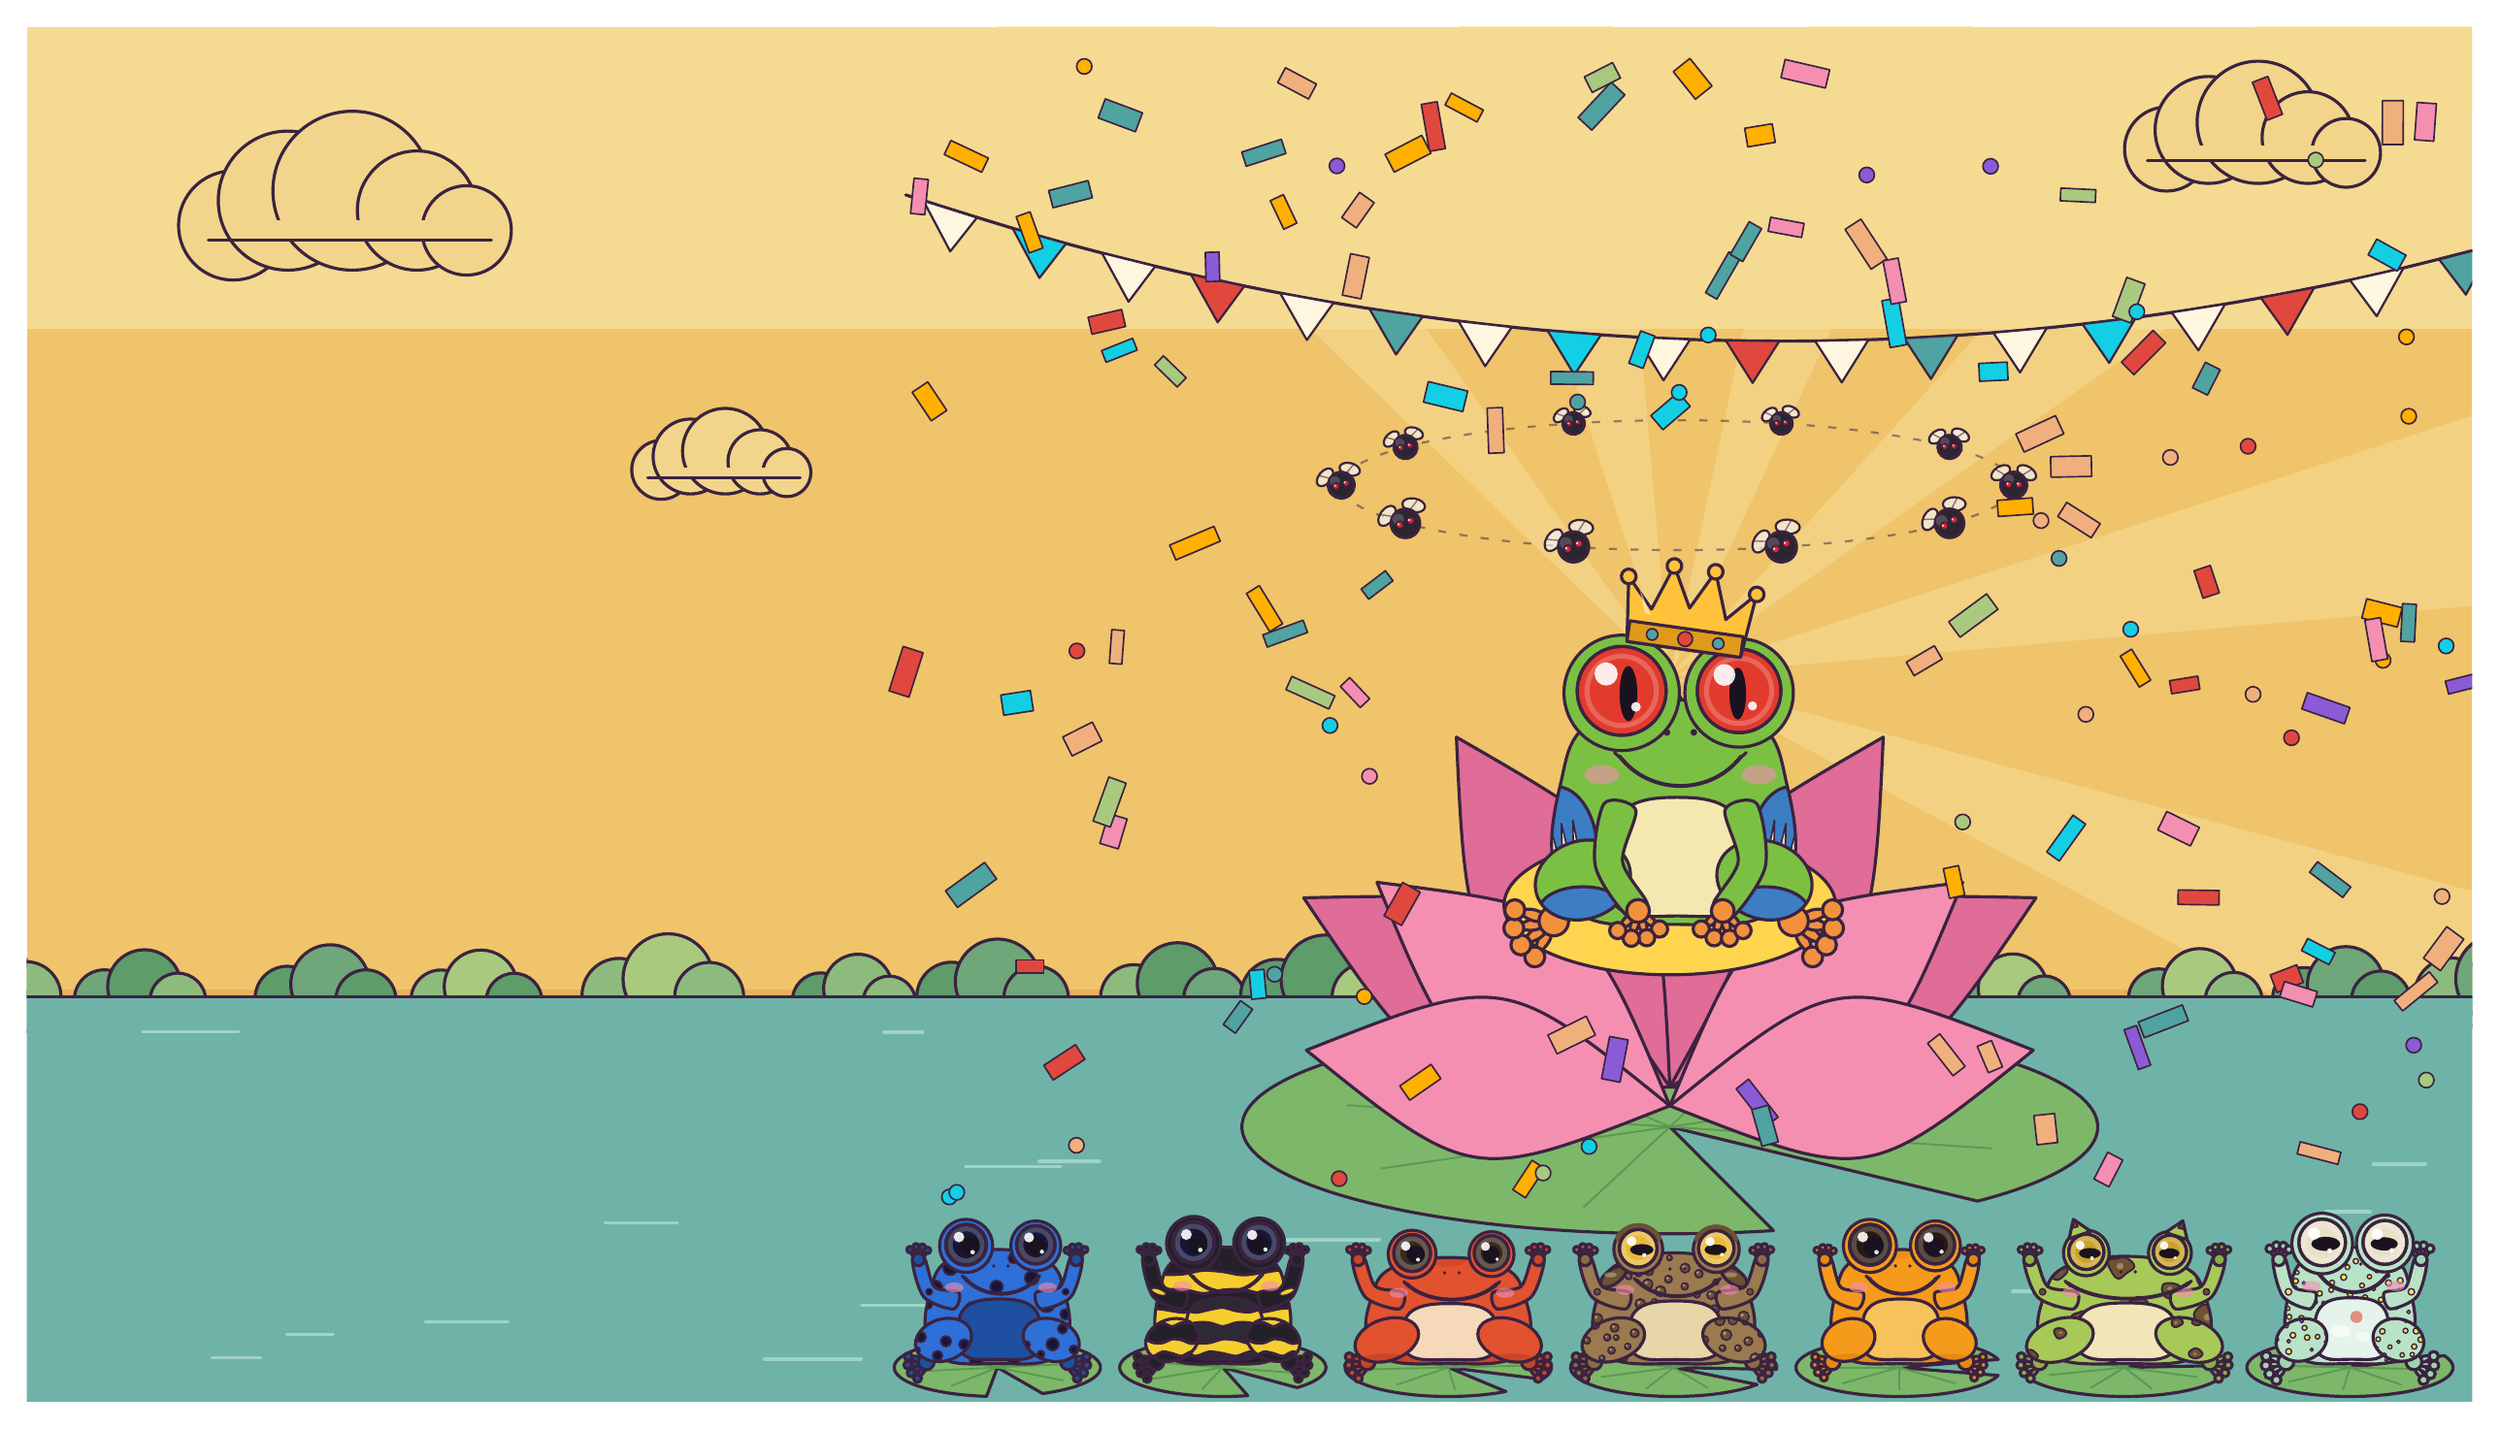
\begin{tikzpicture}
\clip (0,0) rectangle (32,18);
\fill[sky] (0,0) rectangle (32,18);
\fill[skyhi] (0,14.04) rectangle (32,18);
\fill[skylow] (0,0) rectangle (32,5.4);
\fill[skyhi, opacity=0.6] (21.5,9.5) -- (39.159,0.111) -- (40.819,4.324) -- cycle;
\fill[skyhi, opacity=0.6] (21.5,9.5) -- (41.424,11.243) -- (40.521,15.68) -- cycle;
\fill[skyhi, opacity=0.6] (21.5,9.5) -- (37.883,20.972) -- (34.883,24.363) -- cycle;
\fill[skyhi, opacity=0.6] (21.5,9.5) -- (29.952,27.626) -- (25.658,29.063) -- cycle;
\fill[skyhi, opacity=0.6] (21.5,9.5) -- (19.757,29.424) -- (15.32,28.521) -- cycle;
\fill[skyhi, opacity=0.6] (21.5,9.5) -- (10.028,25.883) -- (7.113,23.393) -- cycle;
\filldraw[inked,fill=cloud] (2.7,15.4) circle (0.715);
\filldraw[inked,fill=cloud] (3.415,15.725) circle (0.91);
\filldraw[inked,fill=cloud] (4.26,15.855) circle (1.04);
\filldraw[inked,fill=cloud] (5.105,15.595) circle (0.78);
\filldraw[inked,fill=cloud] (5.755,15.335) circle (0.585);
\fill[cloud] (2.7,15.205) rectangle (5.755,15.465);
\draw[ink, line width=1.15pt, line cap=round] (2.375,15.205) -- (6.08,15.205);
\filldraw[inked,fill=cloud] (8.3,12.2) circle (0.385);
\filldraw[inked,fill=cloud] (8.685,12.375) circle (0.49);
\filldraw[inked,fill=cloud] (9.14,12.445) circle (0.56);
\filldraw[inked,fill=cloud] (9.595,12.305) circle (0.42);
\filldraw[inked,fill=cloud] (9.945,12.165) circle (0.315);
\fill[cloud] (8.3,12.095) rectangle (9.945,12.235);
\draw[ink, line width=1.15pt, line cap=round] (8.125,12.095) -- (10.12,12.095);
\filldraw[inked,fill=cloud] (28,16.4) circle (0.55);
\filldraw[inked,fill=cloud] (28.55,16.65) circle (0.7);
\filldraw[inked,fill=cloud] (29.2,16.75) circle (0.8);
\filldraw[inked,fill=cloud] (29.85,16.55) circle (0.6);
\filldraw[inked,fill=cloud] (30.35,16.35) circle (0.45);
\fill[cloud] (28,16.25) rectangle (30.35,16.45);
\draw[ink, line width=1.15pt, line cap=round] (27.75,16.25) -- (30.6,16.25);
\filldraw[inked,fill=greenB] (-1.208,5.327) circle (0.49);
\filldraw[inked,fill=greenB] (-0.555,5.544) circle (0.599);
\filldraw[inked,fill=greenA] (-0.011,5.305) circle (0.457);
\filldraw[inked,fill=greenB] (1.014,5.262) circle (0.393);
\filldraw[inked,fill=greenD] (1.539,5.437) circle (0.481);
\filldraw[inked,fill=greenA] (1.976,5.245) circle (0.367);
\filldraw[inked,fill=greenD] (3.408,5.281) circle (0.421);
\filldraw[inked,fill=greenB] (3.969,5.468) circle (0.515);
\filldraw[inked,fill=greenD] (4.437,5.262) circle (0.393);
\filldraw[inked,fill=greenA] (5.419,5.261) circle (0.392);
\filldraw[inked,fill=greenC] (5.941,5.435) circle (0.479);
\filldraw[inked,fill=greenD] (6.376,5.244) circle (0.366);
\filldraw[inked,fill=greenA] (7.748,5.322) circle (0.483);
\filldraw[inked,fill=greenC] (8.392,5.537) circle (0.59);
\filldraw[inked,fill=greenA] (8.929,5.301) circle (0.451);
\filldraw[inked,fill=greenD] (10.385,5.246) circle (0.369);
\filldraw[inked,fill=greenA] (10.877,5.409) circle (0.45);
\filldraw[inked,fill=greenA] (11.286,5.229) circle (0.344);
\filldraw[inked,fill=greenD] (12.099,5.302) circle (0.453);
\filldraw[inked,fill=greenB] (12.704,5.504) circle (0.554);
\filldraw[inked,fill=greenB] (13.207,5.282) circle (0.423);
\filldraw[inked,fill=greenA] (14.483,5.289) circle (0.433);
\filldraw[inked,fill=greenD] (15.06,5.481) circle (0.529);
\filldraw[inked,fill=greenB] (15.541,5.269) circle (0.404);
\filldraw[inked,fill=greenD] (16.36,5.317) circle (0.476);
\filldraw[inked,fill=greenD] (16.995,5.529) circle (0.582);
\filldraw[inked,fill=greenC] (17.524,5.296) circle (0.444);
\filldraw[inked,fill=greenD] (18.806,5.317) circle (0.475);
\filldraw[inked,fill=greenB] (19.44,5.528) circle (0.581);
\filldraw[inked,fill=greenB] (19.968,5.296) circle (0.444);
\filldraw[inked,fill=greenC] (21.244,5.249) circle (0.373);
\filldraw[inked,fill=greenC] (21.742,5.415) circle (0.456);
\filldraw[inked,fill=greenD] (22.156,5.232) circle (0.348);
\filldraw[inked,fill=greenB] (23.273,5.258) circle (0.387);
\filldraw[inked,fill=greenC] (23.788,5.43) circle (0.473);
\filldraw[inked,fill=greenC] (24.218,5.241) circle (0.361);
\filldraw[inked,fill=greenB] (25.495,5.246) circle (0.37);
\filldraw[inked,fill=greenC] (25.988,5.411) circle (0.452);
\filldraw[inked,fill=greenB] (26.399,5.23) circle (0.345);
\filldraw[inked,fill=greenB] (27.9,5.267) circle (0.4);
\filldraw[inked,fill=greenC] (28.434,5.444) circle (0.489);
\filldraw[inked,fill=greenA] (28.878,5.249) circle (0.373);
\filldraw[inked,fill=greenD] (29.798,5.274) circle (0.411);
\filldraw[inked,fill=greenB] (30.345,5.457) circle (0.502);
\filldraw[inked,fill=greenD] (30.802,5.256) circle (0.383);
\filldraw[inked,fill=greenA] (31.73,5.324) circle (0.486);
\filldraw[inked,fill=greenB] (32.378,5.54) circle (0.594);
\filldraw[inked,fill=greenB] (32.918,5.302) circle (0.454);
\filldraw[inked,fill=water] (-0.5,-0.5) rectangle (32.5,5.3);
\draw[waterlight, line width=1.3pt, line cap=round] (9.651,0.559) -- (10.916,0.559);
\draw[waterlight, line width=1.3pt, line cap=round] (10.925,1.266) -- (11.861,1.266);
\draw[waterlight, line width=1.3pt, line cap=round] (7.567,2.345) -- (8.513,2.345);
\draw[waterlight, line width=1.3pt, line cap=round] (13.248,3.148) -- (14.037,3.148);
\draw[waterlight, line width=1.3pt, line cap=round] (3.401,0.884) -- (4.007,0.884);
\draw[waterlight, line width=1.3pt, line cap=round] (16.389,2.121) -- (17.697,2.121);
\draw[waterlight, line width=1.3pt, line cap=round] (15.9,3.687) -- (17.38,3.687);
\draw[waterlight, line width=1.3pt, line cap=round] (2.421,0.576) -- (3.061,0.576);
\draw[waterlight, line width=1.3pt, line cap=round] (12.283,3.082) -- (13.527,3.082);
\draw[waterlight, line width=1.3pt, line cap=round] (11.219,4.842) -- (11.722,4.842);
\draw[waterlight, line width=1.3pt, line cap=round] (25.988,1.445) -- (27.363,1.445);
\draw[waterlight, line width=1.3pt, line cap=round] (1.51,4.843) -- (2.77,4.843);
\draw[waterlight, line width=1.3pt, line cap=round] (30.709,3.11) -- (31.387,3.11);
\draw[waterlight, line width=1.3pt, line cap=round] (30.081,2.487) -- (30.664,2.487);
\draw[waterlight, line width=1.3pt, line cap=round] (18.965,2.737) -- (19.938,2.737);
\draw[waterlight, line width=1.3pt, line cap=round] (5.213,1.049) -- (6.294,1.049);
\draw[ink, line width=1.15pt, line cap=round, line join=round] plot[smooth, tension=0.6] coordinates {(11.5,15.8) (13.25,15.261) (15,14.811) (16.75,14.45) (18.5,14.178) (20.25,13.994) (22,13.9) (23.75,13.894) (25.5,13.978) (27.25,14.15) (29,14.411) (30.75,14.761) (32.5,15.2)};
\filldraw[inked,fill=cream,line width=0.8pt] (11.733,15.723) -- (12.433,15.502) -- (12.083,15.06) -- cycle;
\filldraw[inked,fill=cyan,line width=0.8pt] (12.9,15.362) -- (13.6,15.164) -- (13.25,14.711) -- cycle;
\filldraw[inked,fill=cream,line width=0.8pt] (14.067,15.04) -- (14.767,14.866) -- (14.417,14.401) -- cycle;
\filldraw[inked,fill=red,line width=0.8pt] (15.233,14.758) -- (15.933,14.607) -- (15.583,14.131) -- cycle;
\filldraw[inked,fill=cream,line width=0.8pt] (16.4,14.515) -- (17.1,14.388) -- (16.75,13.9) -- cycle;
\filldraw[inked,fill=teal,line width=0.8pt] (17.567,14.312) -- (18.267,14.209) -- (17.917,13.709) -- cycle;
\filldraw[inked,fill=cream,line width=0.8pt] (18.733,14.148) -- (19.433,14.069) -- (19.083,13.557) -- cycle;
\filldraw[inked,fill=cyan,line width=0.8pt] (19.9,14.024) -- (20.6,13.968) -- (20.25,13.444) -- cycle;
\filldraw[inked,fill=cream,line width=0.8pt] (21.067,13.939) -- (21.767,13.907) -- (21.417,13.372) -- cycle;
\filldraw[inked,fill=red,line width=0.8pt] (22.233,13.894) -- (22.933,13.886) -- (22.583,13.338) -- cycle;
\filldraw[inked,fill=cream,line width=0.8pt] (23.4,13.888) -- (24.1,13.904) -- (23.75,13.344) -- cycle;
\filldraw[inked,fill=teal,line width=0.8pt] (24.567,13.922) -- (25.267,13.962) -- (24.917,13.39) -- cycle;
\filldraw[inked,fill=cream,line width=0.8pt] (25.733,13.996) -- (26.433,14.059) -- (26.083,13.475) -- cycle;
\filldraw[inked,fill=cyan,line width=0.8pt] (26.9,14.108) -- (27.6,14.195) -- (27.25,13.6) -- cycle;
\filldraw[inked,fill=cream,line width=0.8pt] (28.067,14.261) -- (28.767,14.371) -- (28.417,13.764) -- cycle;
\filldraw[inked,fill=red,line width=0.8pt] (29.233,14.453) -- (29.933,14.587) -- (29.583,13.968) -- cycle;
\filldraw[inked,fill=cream,line width=0.8pt] (30.4,14.684) -- (31.1,14.842) -- (30.75,14.211) -- cycle;
\filldraw[inked,fill=teal,line width=0.8pt] (31.567,14.955) -- (32.267,15.136) -- (31.917,14.494) -- cycle;
\filldraw[inked,fill=pad] (21.5,3.6) -- ($(21.5,3.6)+(316:5.6 and 1.4)$) arc[start angle=316, end angle=644, x radius=5.6, y radius=1.4] -- cycle;
\draw[paddark, line width=0.7pt] (21.5,3.6) -- (25.719,3.317);
\draw[paddark, line width=0.7pt] (21.5,3.6) -- (25.283,4.146);
\draw[paddark, line width=0.7pt] (21.5,3.6) -- (22.631,4.655);
\draw[paddark, line width=0.7pt] (21.5,3.6) -- (19.316,4.546);
\draw[paddark, line width=0.7pt] (21.5,3.6) -- (17.281,3.883);
\draw[paddark, line width=0.7pt] (21.5,3.6) -- (17.717,3.054);
\draw[paddark, line width=0.7pt] (21.5,3.6) -- (20.369,2.545);
\fill[padlight, opacity=0.6] (19.54,4.09) ellipse (1.232 and 0.224);
\begin{scope}[shift={(21.5,3.7)}, rotate=0, xscale=3.5, yscale=3.5]
\filldraw[inked,fill=lotusdark] (0,0.12) .. controls (0.491,0.847) .. (1.369,0.828) .. controls (0.877,0.101) .. (0,0.12) -- cycle;
\filldraw[inked,fill=lotusdark] (0,0.12) .. controls (0.041,0.993) .. (0.798,1.429) .. controls (0.758,0.556) .. (0,0.12) -- cycle;
\filldraw[inked,fill=lotusdark] (0,0.12) .. controls (-0.42,0.885) .. (0,1.65) .. controls (0.42,0.885) .. (0,0.12) -- cycle;
\filldraw[inked,fill=lotusdark] (0,0.12) .. controls (-0.758,0.556) .. (-0.798,1.429) .. controls (-0.041,0.993) .. (0,0.12) -- cycle;
\filldraw[inked,fill=lotusdark] (0,0.12) .. controls (-0.877,0.101) .. (-1.369,0.828) .. controls (-0.491,0.847) .. (0,0.12) -- cycle;
\filldraw[inked,fill=lotus] (0,0.05) .. controls (0.305,0.786) .. (1.095,0.886) .. controls (0.79,0.15) .. (0,0.05) -- cycle;
\filldraw[inked,fill=lotus] (0,0.05) .. controls (-0.79,0.15) .. (-1.095,0.886) .. controls (-0.305,0.786) .. (0,0.05) -- cycle;
\filldraw[inked,fill=lotuscentre] (0,0.8) ellipse (0.62 and 0.26);
\fill[lotusseed] (-0.3,0.82) circle (0.06);
\fill[lotusseed] (0,0.82) circle (0.06);
\fill[lotusseed] (0.3,0.82) circle (0.06);
\end{scope}
\draw[ink, line width=0.8pt, dash pattern=on 3pt off 5pt, opacity=0.5] (21.6,12.0) ellipse (4.4 and 0.85);
\begin{scope}[shift={(25.16,12.5)}, rotate=3.6, xscale=0.305, yscale=0.305]
\filldraw[inked,fill=flywing,rotate around={32:(-0.5,0.48)},fill opacity=0.65,line width=0.8pt] (-0.5,0.48) ellipse (0.4 and 0.24);
\draw[ink, line width=0.5pt, opacity=0.6] (-0.22,0.32) -- (-0.72,0.62);
\filldraw[inked,fill=flywing,rotate around={-32:(0.5,0.48)},fill opacity=0.65,line width=0.8pt] (0.5,0.48) ellipse (0.4 and 0.24);
\draw[ink, line width=0.5pt, opacity=0.6] (0.22,0.32) -- (0.72,0.62);
\filldraw[inked,fill=flybody] (0,0) circle (0.5);
\fill[white, opacity=0.18] (-0.18,0.22) circle (0.2);
\filldraw[inked,fill=flyeye,line width=0.6pt] (-0.2,0.02) circle (0.13);
\fill[white, opacity=0.9] (-0.24,0.06) circle (0.04);
\filldraw[inked,fill=flyeye,line width=0.6pt] (0.2,0.02) circle (0.13);
\fill[white, opacity=0.9] (0.16,0.06) circle (0.04);
\end{scope}
\begin{scope}[shift={(22.96,12.808)}, rotate=7.2, xscale=0.283, yscale=0.283]
\filldraw[inked,fill=flywing,rotate around={32:(-0.5,0.48)},fill opacity=0.65,line width=0.8pt] (-0.5,0.48) ellipse (0.4 and 0.24);
\draw[ink, line width=0.5pt, opacity=0.6] (-0.22,0.32) -- (-0.72,0.62);
\filldraw[inked,fill=flywing,rotate around={-32:(0.5,0.48)},fill opacity=0.65,line width=0.8pt] (0.5,0.48) ellipse (0.4 and 0.24);
\draw[ink, line width=0.5pt, opacity=0.6] (0.22,0.32) -- (0.72,0.62);
\filldraw[inked,fill=flybody] (0,0) circle (0.5);
\fill[white, opacity=0.18] (-0.18,0.22) circle (0.2);
\filldraw[inked,fill=flyeye,line width=0.6pt] (-0.2,0.02) circle (0.13);
\fill[white, opacity=0.9] (-0.24,0.06) circle (0.04);
\filldraw[inked,fill=flyeye,line width=0.6pt] (0.2,0.02) circle (0.13);
\fill[white, opacity=0.9] (0.16,0.06) circle (0.04);
\end{scope}
\begin{scope}[shift={(20.24,12.808)}, rotate=10.8, xscale=0.283, yscale=0.283]
\filldraw[inked,fill=flywing,rotate around={32:(-0.5,0.48)},fill opacity=0.65,line width=0.8pt] (-0.5,0.48) ellipse (0.4 and 0.24);
\draw[ink, line width=0.5pt, opacity=0.6] (-0.22,0.32) -- (-0.72,0.62);
\filldraw[inked,fill=flywing,rotate around={-32:(0.5,0.48)},fill opacity=0.65,line width=0.8pt] (0.5,0.48) ellipse (0.4 and 0.24);
\draw[ink, line width=0.5pt, opacity=0.6] (0.22,0.32) -- (0.72,0.62);
\filldraw[inked,fill=flybody] (0,0) circle (0.5);
\fill[white, opacity=0.18] (-0.18,0.22) circle (0.2);
\filldraw[inked,fill=flyeye,line width=0.6pt] (-0.2,0.02) circle (0.13);
\fill[white, opacity=0.9] (-0.24,0.06) circle (0.04);
\filldraw[inked,fill=flyeye,line width=0.6pt] (0.2,0.02) circle (0.13);
\fill[white, opacity=0.9] (0.16,0.06) circle (0.04);
\end{scope}
\begin{scope}[shift={(18.04,12.5)}, rotate=14.4, xscale=0.305, yscale=0.305]
\filldraw[inked,fill=flywing,rotate around={32:(-0.5,0.48)},fill opacity=0.65,line width=0.8pt] (-0.5,0.48) ellipse (0.4 and 0.24);
\draw[ink, line width=0.5pt, opacity=0.6] (-0.22,0.32) -- (-0.72,0.62);
\filldraw[inked,fill=flywing,rotate around={-32:(0.5,0.48)},fill opacity=0.65,line width=0.8pt] (0.5,0.48) ellipse (0.4 and 0.24);
\draw[ink, line width=0.5pt, opacity=0.6] (0.22,0.32) -- (0.72,0.62);
\filldraw[inked,fill=flybody] (0,0) circle (0.5);
\fill[white, opacity=0.18] (-0.18,0.22) circle (0.2);
\filldraw[inked,fill=flyeye,line width=0.6pt] (-0.2,0.02) circle (0.13);
\fill[white, opacity=0.9] (-0.24,0.06) circle (0.04);
\filldraw[inked,fill=flyeye,line width=0.6pt] (0.2,0.02) circle (0.13);
\fill[white, opacity=0.9] (0.16,0.06) circle (0.04);
\end{scope}
\begin{scope}[shift={(17.2,12)}, rotate=18, xscale=0.34, yscale=0.34]
\filldraw[inked,fill=flywing,rotate around={32:(-0.5,0.48)},fill opacity=0.65,line width=0.8pt] (-0.5,0.48) ellipse (0.4 and 0.24);
\draw[ink, line width=0.5pt, opacity=0.6] (-0.22,0.32) -- (-0.72,0.62);
\filldraw[inked,fill=flywing,rotate around={-32:(0.5,0.48)},fill opacity=0.65,line width=0.8pt] (0.5,0.48) ellipse (0.4 and 0.24);
\draw[ink, line width=0.5pt, opacity=0.6] (0.22,0.32) -- (0.72,0.62);
\filldraw[inked,fill=flybody] (0,0) circle (0.5);
\fill[white, opacity=0.18] (-0.18,0.22) circle (0.2);
\filldraw[inked,fill=flyeye,line width=0.6pt] (-0.2,0.02) circle (0.13);
\fill[white, opacity=0.9] (-0.24,0.06) circle (0.04);
\filldraw[inked,fill=flyeye,line width=0.6pt] (0.2,0.02) circle (0.13);
\fill[white, opacity=0.9] (0.16,0.06) circle (0.04);
\end{scope}
\begin{scope}[shift={(21.55,6.25)}, rotate=0, xscale=0.88, yscale=0.88]
\filldraw[inked,fill=limefeet] (-1.782,0.05) .. controls (-1.827,-0.268) .. (-2.066,-0.483) .. controls (-2.021,-0.165) .. (-1.782,0.05) -- cycle;
\filldraw[inked,fill=limefeet] (-2.066,-0.483) circle (0.149);
\filldraw[inked,fill=limefeet] (-1.782,0.05) .. controls (-1.962,-0.217) .. (-2.271,-0.305) .. controls (-2.091,-0.039) .. (-1.782,0.05) -- cycle;
\filldraw[inked,fill=limefeet] (-2.271,-0.305) circle (0.149);
\filldraw[inked,fill=limefeet] (-1.782,0.05) .. controls (-2.06,-0.111) .. (-2.377,-0.055) .. controls (-2.099,0.106) .. (-1.782,0.05) -- cycle;
\filldraw[inked,fill=limefeet] (-2.377,-0.055) circle (0.149);
\filldraw[inked,fill=limefeet] (-1.782,0.05) .. controls (-2.103,0.028) .. (-2.363,0.217) .. controls (-2.042,0.239) .. (-1.782,0.05) -- cycle;
\filldraw[inked,fill=limefeet] (-2.363,0.217) circle (0.149);
\filldraw[inked,fill=limefeet] (-1.782,0.05) circle (0.22);
\filldraw[inked,fill=limefeet] (1.782,0.05) .. controls (2.021,-0.165) .. (2.066,-0.483) .. controls (1.827,-0.268) .. (1.782,0.05) -- cycle;
\filldraw[inked,fill=limefeet] (2.066,-0.483) circle (0.149);
\filldraw[inked,fill=limefeet] (1.782,0.05) .. controls (2.091,-0.039) .. (2.271,-0.305) .. controls (1.962,-0.217) .. (1.782,0.05) -- cycle;
\filldraw[inked,fill=limefeet] (2.271,-0.305) circle (0.149);
\filldraw[inked,fill=limefeet] (1.782,0.05) .. controls (2.099,0.106) .. (2.377,-0.055) .. controls (2.06,-0.111) .. (1.782,0.05) -- cycle;
\filldraw[inked,fill=limefeet] (2.377,-0.055) circle (0.149);
\filldraw[inked,fill=limefeet] (1.782,0.05) .. controls (2.042,0.239) .. (2.363,0.217) .. controls (2.103,0.028) .. (1.782,0.05) -- cycle;
\filldraw[inked,fill=limefeet] (2.363,0.217) circle (0.149);
\filldraw[inked,fill=limefeet] (1.782,0.05) circle (0.22);
\fill[limeskin] plot[smooth cycle, tension=0.7] coordinates {(0,0) (1.305,0.105) (1.782,0.84) (1.692,2.047) (1.26,2.993) (0,3.339) (-1.26,2.993) (-1.692,2.047) (-1.782,0.84) (-1.305,0.105)};
\begin{scope}\clip plot[smooth cycle, tension=0.7] coordinates {(0,0) (1.305,0.105) (1.782,0.84) (1.692,2.047) (1.26,2.993) (0,3.339) (-1.26,2.993) (-1.692,2.047) (-1.782,0.84) (-1.305,0.105)};
\filldraw[inked,fill=limemark] (-1.75,1.05) ellipse (0.62 and 1);
\filldraw[inked,fill=limebelly,line width=0.6pt] (-1.38,0.45) .. controls (-1.49,0.995) .. (-1.5,1.55) .. controls (-1.39,1.005) .. (-1.38,0.45) -- cycle;
\filldraw[inked,fill=limebelly,line width=0.6pt] (-1.55,0.6) .. controls (-1.66,1.043) .. (-1.67,1.5) .. controls (-1.56,1.057) .. (-1.55,0.6) -- cycle;
\filldraw[inked,fill=limebelly,line width=0.6pt] (-1.72,0.75) .. controls (-1.829,1.092) .. (-1.84,1.45) .. controls (-1.731,1.108) .. (-1.72,0.75) -- cycle;
\filldraw[inked,fill=limemark] (1.75,1.05) ellipse (0.62 and 1);
\filldraw[inked,fill=limebelly,line width=0.6pt] (1.38,0.45) .. controls (1.39,1.005) .. (1.5,1.55) .. controls (1.49,0.995) .. (1.38,0.45) -- cycle;
\filldraw[inked,fill=limebelly,line width=0.6pt] (1.55,0.6) .. controls (1.56,1.057) .. (1.67,1.5) .. controls (1.66,1.043) .. (1.55,0.6) -- cycle;
\filldraw[inked,fill=limebelly,line width=0.6pt] (1.72,0.75) .. controls (1.731,1.108) .. (1.84,1.45) .. controls (1.829,1.092) .. (1.72,0.75) -- cycle;
\end{scope}
\draw[inked] plot[smooth cycle, tension=0.7] coordinates {(0,0) (1.305,0.105) (1.782,0.84) (1.692,2.047) (1.26,2.993) (0,3.339) (-1.26,2.993) (-1.692,2.047) (-1.782,0.84) (-1.305,0.105)};
\fill[limebelly] plot[smooth cycle, tension=0.7] coordinates {(0.05,0.126) (0.905,0.231) (1.085,0.945) (0.86,1.68) (0.05,1.89) (-0.76,1.68) (-0.985,0.945) (-0.805,0.231)};
\draw[inked] plot[smooth cycle, tension=0.7] coordinates {(0.05,0.126) (0.905,0.231) (1.085,0.945) (0.86,1.68) (0.05,1.89) (-0.76,1.68) (-0.985,0.945) (-0.805,0.231)};
\fill[limeskin] [rotate around={18:(-1.35,0.66)}] (-1.35,0.66) ellipse (0.72 and 0.58);
\begin{scope}\clip [rotate around={18:(-1.35,0.66)}] (-1.35,0.66) ellipse (0.72 and 0.58);
\filldraw[inked,fill=limemark] (-1.35,0.21) ellipse (0.648 and 0.35);
\end{scope}
\draw[inked] [rotate around={18:(-1.35,0.66)}] (-1.35,0.66) ellipse (0.72 and 0.58);
\fill[limeskin] [rotate around={-18:(1.35,0.66)}] (1.35,0.66) ellipse (0.72 and 0.58);
\begin{scope}\clip [rotate around={-18:(1.35,0.66)}] (1.35,0.66) ellipse (0.72 and 0.58);
\filldraw[inked,fill=limemark] (1.35,0.21) ellipse (0.648 and 0.35);
\end{scope}
\draw[inked] [rotate around={-18:(1.35,0.66)}] (1.35,0.66) ellipse (0.72 and 0.58);
\filldraw[inked,fill=limeskin] plot[smooth cycle, tension=0.5] coordinates {(-0.564,1.705) (-0.76,0.935) (-0.385,0.289) (-0.675,0.111) (-1.164,0.865) (-1.036,1.795)};
\filldraw[inked,fill=limefeet] (-0.53,0.2) .. controls (-0.318,0.127) .. (-0.21,-0.069) .. controls (-0.421,0.004) .. (-0.53,0.2) -- cycle;
\filldraw[inked,fill=limefeet] (-0.21,-0.069) circle (0.121);
\filldraw[inked,fill=limefeet] (-0.53,0.2) .. controls (-0.389,0.026) .. (-0.401,-0.198) .. controls (-0.541,-0.024) .. (-0.53,0.2) -- cycle;
\filldraw[inked,fill=limefeet] (-0.401,-0.198) circle (0.121);
\filldraw[inked,fill=limefeet] (-0.53,0.2) .. controls (-0.503,-0.022) .. (-0.631,-0.206) .. controls (-0.658,0.016) .. (-0.53,0.2) -- cycle;
\filldraw[inked,fill=limefeet] (-0.631,-0.206) circle (0.121);
\filldraw[inked,fill=limefeet] (-0.53,0.2) .. controls (-0.625,-0.003) .. (-0.831,-0.091) .. controls (-0.736,0.112) .. (-0.53,0.2) -- cycle;
\filldraw[inked,fill=limefeet] (-0.831,-0.091) circle (0.121);
\filldraw[inked,fill=limefeet] (-0.53,0.2) circle (0.17);
\filldraw[inked,fill=limeskin] plot[smooth cycle, tension=0.5] coordinates {(1.236,1.795) (1.364,0.865) (0.875,0.111) (0.585,0.289) (0.96,0.935) (0.764,1.705)};
\filldraw[inked,fill=limefeet] (0.73,0.2) .. controls (0.621,0.004) .. (0.41,-0.069) .. controls (0.518,0.127) .. (0.73,0.2) -- cycle;
\filldraw[inked,fill=limefeet] (0.41,-0.069) circle (0.121);
\filldraw[inked,fill=limefeet] (0.73,0.2) .. controls (0.741,-0.024) .. (0.601,-0.198) .. controls (0.589,0.026) .. (0.73,0.2) -- cycle;
\filldraw[inked,fill=limefeet] (0.601,-0.198) circle (0.121);
\filldraw[inked,fill=limefeet] (0.73,0.2) .. controls (0.858,0.016) .. (0.831,-0.206) .. controls (0.703,-0.022) .. (0.73,0.2) -- cycle;
\filldraw[inked,fill=limefeet] (0.831,-0.206) circle (0.121);
\filldraw[inked,fill=limefeet] (0.73,0.2) .. controls (0.936,0.112) .. (1.031,-0.091) .. controls (0.825,-0.003) .. (0.73,0.2) -- cycle;
\filldraw[inked,fill=limefeet] (1.031,-0.091) circle (0.121);
\filldraw[inked,fill=limefeet] (0.73,0.2) circle (0.17);
\fill[ink] (-0.1,2.856) circle (0.05);
\fill[blush, opacity=0.6] (-1.07,2.226) ellipse (0.26 and 0.14);
\fill[ink] (0.3,2.856) circle (0.05);
\fill[blush, opacity=0.6] (1.27,2.226) ellipse (0.26 and 0.14);
\draw[ink, line width=1.438pt, line cap=round] (-0.8,2.495) .. controls (-0.35,1.915) and (0.55,1.915) .. (1,2.495);
\draw[ink, line width=1.15pt, line cap=round] (-0.72,2.415) -- (-0.88,2.555);
\draw[ink, line width=1.15pt, line cap=round] (0.92,2.415) -- (1.08,2.555);
\filldraw[inked,fill=limeskin] (-0.773,3.444) circle (0.858);
\filldraw[inked,fill=limeeye] (-0.773,3.474) circle (0.661);
\draw[white, opacity=0.22, line width=1.84pt] (-0.773,3.474) circle (0.516);
\fill[pupil] (-0.673,3.434) ellipse (0.132 and 0.41);
\fill[white, opacity=0.9] (-1.004,3.725) circle (0.172);
\fill[white, opacity=0.9] (-0.561,3.236) circle (0.073);
\draw[inked] (-0.773,3.474) circle (0.661);
\filldraw[inked,fill=limeskin] (0.973,3.444) circle (0.807);
\filldraw[inked,fill=limeeye] (0.973,3.474) circle (0.622);
\draw[white, opacity=0.22, line width=1.84pt] (0.973,3.474) circle (0.485);
\fill[pupil] (0.953,3.434) ellipse (0.124 and 0.385);
\fill[white, opacity=0.9] (0.755,3.71) circle (0.162);
\fill[white, opacity=0.9] (1.172,3.25) circle (0.068);
\draw[inked] (0.973,3.474) circle (0.622);
\begin{scope}[shift={(0.15,4.091)}, rotate=-8, xscale=1, yscale=1]
\filldraw[inked,fill=crown] (-0.853,0) -- (0.853,0) -- (0.961,0.961) -- (0.558,0.527) -- (0.31,1.209) -- (0,0.62) -- (-0.31,1.209) -- (-0.558,0.527) -- (-0.961,0.961) -- cycle;
\filldraw[inked,fill=crowndark] (-0.853,0) rectangle (0.853,0.31);
\filldraw[inked,fill=crown] (-0.961,0.961) circle (0.109);
\filldraw[inked,fill=crown] (0.961,0.961) circle (0.109);
\filldraw[inked,fill=crown] (-0.31,1.209) circle (0.109);
\filldraw[inked,fill=crown] (0.31,1.209) circle (0.109);
\filldraw[inked,fill=jewel,line width=0.6pt] (0,0.155) circle (0.109);
\filldraw[inked,fill=jewelb,line width=0.6pt] (-0.496,0.155) circle (0.085);
\filldraw[inked,fill=jewelb,line width=0.6pt] (0.496,0.155) circle (0.085);
\fill[white, opacity=0.5] (-0.651,0.465) -- (-0.558,0.434) -- (-0.775,0.806) -- cycle;
\end{scope}
\end{scope}
\begin{scope}[shift={(21.5,3.7)}, rotate=0, xscale=3.5, yscale=3.5]
\filldraw[inked,fill=lotus] (0,0.05) .. controls (0.619,0.55) .. (1.359,0.258) .. controls (0.74,-0.241) .. (0,0.05) -- cycle;
\filldraw[inked,fill=lotus] (0,0.05) .. controls (-0.74,-0.241) .. (-1.359,0.258) .. controls (-0.619,0.55) .. (0,0.05) -- cycle;
\end{scope}
\begin{scope}[shift={(26,12)}, rotate=0, xscale=0.34, yscale=0.34]
\filldraw[inked,fill=flywing,rotate around={32:(-0.5,0.48)},fill opacity=0.65,line width=0.8pt] (-0.5,0.48) ellipse (0.4 and 0.24);
\draw[ink, line width=0.5pt, opacity=0.6] (-0.22,0.32) -- (-0.72,0.62);
\filldraw[inked,fill=flywing,rotate around={-32:(0.5,0.48)},fill opacity=0.65,line width=0.8pt] (0.5,0.48) ellipse (0.4 and 0.24);
\draw[ink, line width=0.5pt, opacity=0.6] (0.22,0.32) -- (0.72,0.62);
\filldraw[inked,fill=flybody] (0,0) circle (0.5);
\fill[white, opacity=0.18] (-0.18,0.22) circle (0.2);
\filldraw[inked,fill=flyeye,line width=0.6pt] (-0.2,0.02) circle (0.13);
\fill[white, opacity=0.9] (-0.24,0.06) circle (0.04);
\filldraw[inked,fill=flyeye,line width=0.6pt] (0.2,0.02) circle (0.13);
\fill[white, opacity=0.9] (0.16,0.06) circle (0.04);
\end{scope}
\begin{scope}[shift={(18.04,11.5)}, rotate=21.6, xscale=0.375, yscale=0.375]
\filldraw[inked,fill=flywing,rotate around={32:(-0.5,0.48)},fill opacity=0.65,line width=0.8pt] (-0.5,0.48) ellipse (0.4 and 0.24);
\draw[ink, line width=0.5pt, opacity=0.6] (-0.22,0.32) -- (-0.72,0.62);
\filldraw[inked,fill=flywing,rotate around={-32:(0.5,0.48)},fill opacity=0.65,line width=0.8pt] (0.5,0.48) ellipse (0.4 and 0.24);
\draw[ink, line width=0.5pt, opacity=0.6] (0.22,0.32) -- (0.72,0.62);
\filldraw[inked,fill=flybody] (0,0) circle (0.5);
\fill[white, opacity=0.18] (-0.18,0.22) circle (0.2);
\filldraw[inked,fill=flyeye,line width=0.6pt] (-0.2,0.02) circle (0.13);
\fill[white, opacity=0.9] (-0.24,0.06) circle (0.04);
\filldraw[inked,fill=flyeye,line width=0.6pt] (0.2,0.02) circle (0.13);
\fill[white, opacity=0.9] (0.16,0.06) circle (0.04);
\end{scope}
\begin{scope}[shift={(20.24,11.192)}, rotate=25.2, xscale=0.397, yscale=0.397]
\filldraw[inked,fill=flywing,rotate around={32:(-0.5,0.48)},fill opacity=0.65,line width=0.8pt] (-0.5,0.48) ellipse (0.4 and 0.24);
\draw[ink, line width=0.5pt, opacity=0.6] (-0.22,0.32) -- (-0.72,0.62);
\filldraw[inked,fill=flywing,rotate around={-32:(0.5,0.48)},fill opacity=0.65,line width=0.8pt] (0.5,0.48) ellipse (0.4 and 0.24);
\draw[ink, line width=0.5pt, opacity=0.6] (0.22,0.32) -- (0.72,0.62);
\filldraw[inked,fill=flybody] (0,0) circle (0.5);
\fill[white, opacity=0.18] (-0.18,0.22) circle (0.2);
\filldraw[inked,fill=flyeye,line width=0.6pt] (-0.2,0.02) circle (0.13);
\fill[white, opacity=0.9] (-0.24,0.06) circle (0.04);
\filldraw[inked,fill=flyeye,line width=0.6pt] (0.2,0.02) circle (0.13);
\fill[white, opacity=0.9] (0.16,0.06) circle (0.04);
\end{scope}
\begin{scope}[shift={(22.96,11.192)}, rotate=28.8, xscale=0.397, yscale=0.397]
\filldraw[inked,fill=flywing,rotate around={32:(-0.5,0.48)},fill opacity=0.65,line width=0.8pt] (-0.5,0.48) ellipse (0.4 and 0.24);
\draw[ink, line width=0.5pt, opacity=0.6] (-0.22,0.32) -- (-0.72,0.62);
\filldraw[inked,fill=flywing,rotate around={-32:(0.5,0.48)},fill opacity=0.65,line width=0.8pt] (0.5,0.48) ellipse (0.4 and 0.24);
\draw[ink, line width=0.5pt, opacity=0.6] (0.22,0.32) -- (0.72,0.62);
\filldraw[inked,fill=flybody] (0,0) circle (0.5);
\fill[white, opacity=0.18] (-0.18,0.22) circle (0.2);
\filldraw[inked,fill=flyeye,line width=0.6pt] (-0.2,0.02) circle (0.13);
\fill[white, opacity=0.9] (-0.24,0.06) circle (0.04);
\filldraw[inked,fill=flyeye,line width=0.6pt] (0.2,0.02) circle (0.13);
\fill[white, opacity=0.9] (0.16,0.06) circle (0.04);
\end{scope}
\begin{scope}[shift={(25.16,11.5)}, rotate=32.4, xscale=0.375, yscale=0.375]
\filldraw[inked,fill=flywing,rotate around={32:(-0.5,0.48)},fill opacity=0.65,line width=0.8pt] (-0.5,0.48) ellipse (0.4 and 0.24);
\draw[ink, line width=0.5pt, opacity=0.6] (-0.22,0.32) -- (-0.72,0.62);
\filldraw[inked,fill=flywing,rotate around={-32:(0.5,0.48)},fill opacity=0.65,line width=0.8pt] (0.5,0.48) ellipse (0.4 and 0.24);
\draw[ink, line width=0.5pt, opacity=0.6] (0.22,0.32) -- (0.72,0.62);
\filldraw[inked,fill=flybody] (0,0) circle (0.5);
\fill[white, opacity=0.18] (-0.18,0.22) circle (0.2);
\filldraw[inked,fill=flyeye,line width=0.6pt] (-0.2,0.02) circle (0.13);
\fill[white, opacity=0.9] (-0.24,0.06) circle (0.04);
\filldraw[inked,fill=flyeye,line width=0.6pt] (0.2,0.02) circle (0.13);
\fill[white, opacity=0.9] (0.16,0.06) circle (0.04);
\end{scope}
\filldraw[inked,fill=violet,line width=0.6pt] (20.848,4.184) -- (20.954,4.737) -- (20.713,4.784) -- (20.606,4.231) -- cycle;
\filldraw[inked,fill=red,line width=0.6pt] (28.067,9.269) -- (28.436,9.329) -- (28.408,9.5) -- (28.039,9.44) -- cycle;
\filldraw[inked,fill=gold,line width=0.6pt] (25.798,11.59) -- (26.258,11.622) -- (26.243,11.834) -- (25.783,11.801) -- cycle;
\filldraw[inked,fill=wallD,line width=0.6pt] (27.132,11.496) -- (26.694,11.775) -- (26.576,11.59) -- (27.014,11.311) -- cycle;
\filldraw[inked,fill=wallD,line width=0.6pt] (26.488,12.104) -- (27.02,12.115) -- (27.014,12.384) -- (26.482,12.373) -- cycle;
\filldraw[inked,fill=wallD,line width=0.6pt] (31.584,5.644) -- (31.89,6.056) -- (31.667,6.221) -- (31.361,5.809) -- cycle;
\filldraw[inked,fill=cyan,line width=0.6pt] (26.596,7.08) -- (26.941,7.562) -- (26.776,7.68) -- (26.431,7.198) -- cycle;
\filldraw[inked,fill=red,line width=0.6pt] (13.741,9.83) circle (0.1);
\filldraw[inked,fill=wallD,line width=0.6pt] (24.341,14.963) -- (24,15.483) -- (23.793,15.348) -- (24.134,14.827) -- cycle;
\filldraw[inked,fill=violet,line width=0.6pt] (15.61,14.669) -- (15.601,15.052) -- (15.421,15.047) -- (15.43,14.665) -- cycle;
\filldraw[inked,fill=cyan,line width=0.6pt] (17.053,8.854) circle (0.1);
\filldraw[inked,fill=red,line width=0.6pt] (28.689,6.693) -- (28.152,6.701) -- (28.149,6.512) -- (28.686,6.504) -- cycle;
\filldraw[inked,fill=red,line width=0.6pt] (27.572,13.446) -- (27.988,13.862) -- (27.824,14.026) -- (27.409,13.61) -- cycle;
\filldraw[inked,fill=greenC,line width=0.6pt] (27.531,14.123) -- (27.718,14.633) -- (27.48,14.721) -- (27.293,14.211) -- cycle;
\filldraw[inked,fill=violet,line width=0.6pt] (27.792,4.408) -- (27.605,4.927) -- (27.444,4.869) -- (27.632,4.35) -- cycle;
\filldraw[inked,fill=gold,line width=0.6pt] (25.359,6.633) -- (25.277,7.02) -- (25.079,6.978) -- (25.16,6.591) -- cycle;
\filldraw[inked,fill=gold,line width=0.6pt] (12.583,16.281) -- (12.092,16.513) -- (12.005,16.329) -- (12.495,16.096) -- cycle;
\filldraw[inked,fill=wallD,line width=0.6pt] (26.357,11.536) circle (0.1);
\filldraw[inked,fill=greenC,line width=0.6pt] (29.952,16.256) circle (0.1);
\filldraw[inked,fill=wallD,line width=0.6pt] (26.575,3.395) -- (26.534,3.775) -- (26.264,3.746) -- (26.306,3.365) -- cycle;
\filldraw[inked,fill=wallD,line width=0.6pt] (13.735,3.358) circle (0.1);
\filldraw[inked,fill=teal,line width=0.6pt] (16.232,9.88) -- (16.759,10.072) -- (16.701,10.232) -- (16.173,10.04) -- cycle;
\filldraw[inked,fill=lotus,line width=0.6pt] (14.282,7.239) -- (14.398,7.629) -- (14.157,7.701) -- (14.041,7.311) -- cycle;
\filldraw[inked,fill=wallD,line width=0.6pt] (17.458,14.439) -- (17.567,14.98) -- (17.323,15.03) -- (17.214,14.488) -- cycle;
\filldraw[inked,fill=cyan,line width=0.6pt] (31.659,9.895) circle (0.1);
\filldraw[inked,fill=cyan,line width=0.6pt] (31.134,15.009) -- (30.751,15.221) -- (30.637,15.015) -- (31.019,14.803) -- cycle;
\filldraw[inked,fill=wallD,line width=0.6pt] (14.328,9.656) -- (14.362,10.096) -- (14.198,10.109) -- (14.165,9.669) -- cycle;
\filldraw[inked,fill=lotus,line width=0.6pt] (17.57,8.189) circle (0.1);
\filldraw[inked,fill=gold,line width=0.6pt] (15.036,11.021) -- (15.617,11.266) -- (15.534,11.461) -- (14.954,11.215) -- cycle;
\filldraw[inked,fill=gold,line width=0.6pt] (22.052,17.226) -- (21.762,17.587) -- (21.545,17.413) -- (21.835,17.052) -- cycle;
\filldraw[inked,fill=wallD,line width=0.6pt] (24.697,9.506) -- (25.064,9.723) -- (24.961,9.898) -- (24.594,9.682) -- cycle;
\filldraw[inked,fill=wallD,line width=0.6pt] (26.944,9) circle (0.1);
\filldraw[inked,fill=teal,line width=0.6pt] (31.244,9.947) -- (31.269,10.44) -- (31.088,10.449) -- (31.063,9.956) -- cycle;
\filldraw[inked,fill=cyan,line width=0.6pt] (27.611,14.27) circle (0.1);
\filldraw[inked,fill=wallD,line width=0.6pt] (29.132,9.262) circle (0.1);
\filldraw[inked,fill=greenC,line width=0.6pt] (31.399,4.212) circle (0.1);
\filldraw[inked,fill=cyan,line width=0.6pt] (27.531,10.113) circle (0.1);
\filldraw[inked,fill=red,line width=0.6pt] (29.445,5.359) -- (29.791,5.491) -- (29.703,5.721) -- (29.357,5.589) -- cycle;
\filldraw[inked,fill=cyan,line width=0.6pt] (12.072,2.682) circle (0.1);
\filldraw[inked,fill=lotus,line width=0.6pt] (28.43,7.519) -- (28.003,7.729) -- (27.884,7.487) -- (28.312,7.277) -- cycle;
\filldraw[inked,fill=greenC,line width=0.6pt] (25.298,10.009) -- (25.794,10.375) -- (25.645,10.577) -- (25.149,10.21) -- cycle;
\filldraw[inked,fill=wallD,line width=0.6pt] (20.025,4.555) -- (20.526,4.802) -- (20.405,5.048) -- (19.904,4.801) -- cycle;
\filldraw[inked,fill=cyan,line width=0.6pt] (20.443,3.343) circle (0.1);
\filldraw[inked,fill=cyan,line width=0.6pt] (21.409,12.725) -- (21.767,13.032) -- (21.609,13.216) -- (21.251,12.91) -- cycle;
\filldraw[inked,fill=red,line width=0.6pt] (17.173,2.921) circle (0.1);
\filldraw[inked,fill=wallD,line width=0.6pt] (28.05,12.363) circle (0.1);
\filldraw[inked,fill=violet,line width=0.6pt] (30.401,9.089) -- (29.843,9.284) -- (29.769,9.071) -- (30.327,8.876) -- cycle;
\filldraw[inked,fill=red,line width=0.6pt] (29.517,16.855) -- (29.325,17.351) -- (29.123,17.273) -- (29.316,16.777) -- cycle;
\filldraw[inked,fill=red,line width=0.6pt] (18.563,16.406) -- (18.455,17.02) -- (18.247,16.984) -- (18.355,16.37) -- cycle;
\filldraw[inked,fill=red,line width=0.6pt] (13.939,13.976) -- (14.378,14.077) -- (14.326,14.3) -- (13.887,14.198) -- cycle;
\filldraw[inked,fill=gold,line width=0.6pt] (19.61,2.67) -- (19.862,3.054) -- (19.697,3.162) -- (19.445,2.778) -- cycle;
\filldraw[inked,fill=red,line width=0.6pt] (29.067,12.509) circle (0.1);
\filldraw[inked,fill=gold,line width=0.6pt] (12.038,12.978) -- (11.789,13.352) -- (11.585,13.216) -- (11.835,12.842) -- cycle;
\filldraw[inked,fill=gold,line width=0.6pt] (13.837,17.482) circle (0.1);
\filldraw[inked,fill=cyan,line width=0.6pt] (18.855,13.232) -- (18.34,13.356) -- (18.276,13.087) -- (18.79,12.963) -- cycle;
\filldraw[inked,fill=lotus,line width=0.6pt] (31.496,16.503) -- (31.531,16.993) -- (31.28,17.01) -- (31.245,16.521) -- cycle;
\filldraw[inked,fill=teal,line width=0.6pt] (27.709,4.766) -- (28.286,4.99) -- (28.206,5.196) -- (27.629,4.972) -- cycle;
\filldraw[inked,fill=teal,line width=0.6pt] (26.593,11.041) circle (0.1);
\filldraw[inked,fill=greenC,line width=0.6pt] (27.075,15.867) -- (26.617,15.889) -- (26.609,15.723) -- (27.067,15.701) -- cycle;
\filldraw[inked,fill=violet,line width=0.6pt] (17.144,16.179) circle (0.1);
\filldraw[inked,fill=gold,line width=0.6pt] (30.833,9.707) circle (0.1);
\filldraw[inked,fill=red,line width=0.6pt] (13.431,4.213) -- (13.847,4.485) -- (13.722,4.676) -- (13.307,4.404) -- cycle;
\filldraw[inked,fill=lotus,line width=0.6pt] (27.247,2.815) -- (27.427,3.165) -- (27.23,3.267) -- (27.05,2.917) -- cycle;
\filldraw[inked,fill=gold,line width=0.6pt] (18.096,3.948) -- (18.504,4.231) -- (18.374,4.418) -- (17.966,4.135) -- cycle;
\filldraw[inked,fill=greenC,line width=0.6pt] (14.178,7.523) -- (14.385,8.098) -- (14.159,8.18) -- (13.952,7.604) -- cycle;
\filldraw[inked,fill=gold,line width=0.6pt] (27.793,9.448) -- (27.542,9.853) -- (27.393,9.761) -- (27.644,9.356) -- cycle;
\filldraw[inked,fill=teal,line width=0.6pt] (16.328,5.597) circle (0.1);
\filldraw[inked,fill=teal,line width=0.6pt] (22.114,14.435) -- (22.422,14.97) -- (22.274,15.055) -- (21.966,14.52) -- cycle;
\filldraw[inked,fill=lotus,line width=0.6pt] (23.257,15.426) -- (22.82,15.507) -- (22.786,15.323) -- (23.223,15.242) -- cycle;
\filldraw[inked,fill=cyan,line width=0.6pt] (30.207,5.881) -- (29.847,6.066) -- (29.766,5.908) -- (30.126,5.723) -- cycle;
\filldraw[inked,fill=violet,line width=0.6pt] (22.917,3.728) -- (22.53,4.224) -- (22.368,4.097) -- (22.754,3.602) -- cycle;
\filldraw[inked,fill=wallD,line width=0.6pt] (30.282,3.266) -- (29.749,3.404) -- (29.709,3.247) -- (30.241,3.109) -- cycle;
\filldraw[inked,fill=teal,line width=0.6pt] (20.499,13.482) -- (19.942,13.488) -- (19.941,13.323) -- (20.497,13.317) -- cycle;
\filldraw[inked,fill=gold,line width=0.6pt] (22.52,16.428) -- (22.88,16.488) -- (22.839,16.731) -- (22.479,16.672) -- cycle;
\filldraw[inked,fill=wallD,line width=0.6pt] (16.876,17.25) -- (16.47,17.465) -- (16.367,17.27) -- (16.773,17.055) -- cycle;
\filldraw[inked,fill=gold,line width=0.6pt] (16.619,15.431) -- (16.442,15.804) -- (16.271,15.723) -- (16.448,15.35) -- cycle;
\filldraw[inked,fill=wallD,line width=0.6pt] (13.679,8.455) -- (14.068,8.651) -- (13.943,8.898) -- (13.555,8.703) -- cycle;
\filldraw[inked,fill=cyan,line width=0.6pt] (22.002,13.966) circle (0.1);
\filldraw[inked,fill=cyan,line width=0.6pt] (25.554,13.36) -- (25.926,13.378) -- (25.914,13.611) -- (25.542,13.593) -- cycle;
\filldraw[inked,fill=teal,line width=0.6pt] (17.56,10.507) -- (17.877,10.748) -- (17.777,10.88) -- (17.46,10.638) -- cycle;
\filldraw[inked,fill=teal,line width=0.6pt] (20.478,16.647) -- (20.911,17.109) -- (20.732,17.276) -- (20.299,16.814) -- cycle;
\filldraw[inked,fill=gold,line width=0.6pt] (16.433,10.186) -- (16.128,10.685) -- (15.959,10.581) -- (16.264,10.082) -- cycle;
\filldraw[inked,fill=gold,line width=0.6pt] (31.139,13.941) circle (0.1);
\filldraw[inked,fill=red,line width=0.6pt] (11.543,9.224) -- (11.728,9.805) -- (11.467,9.889) -- (11.282,9.308) -- cycle;
\filldraw[inked,fill=wallD,line width=0.6pt] (25.853,4.385) -- (25.708,4.73) -- (25.523,4.653) -- (25.668,4.308) -- cycle;
\filldraw[inked,fill=cyan,line width=0.6pt] (24.599,13.839) -- (24.491,14.452) -- (24.275,14.414) -- (24.383,13.801) -- cycle;
\filldraw[inked,fill=gold,line width=0.6pt] (31.084,10.395) -- (30.619,10.513) -- (30.555,10.261) -- (31.019,10.142) -- cycle;
\filldraw[inked,fill=red,line width=0.6pt] (28.691,10.591) -- (28.572,10.949) -- (28.359,10.878) -- (28.478,10.52) -- cycle;
\filldraw[inked,fill=red,line width=0.6pt] (17.989,6.235) -- (18.234,6.671) -- (18.004,6.8) -- (17.759,6.364) -- cycle;
\filldraw[inked,fill=teal,line width=0.6pt] (22.453,14.927) -- (22.701,15.357) -- (22.539,15.45) -- (22.291,15.021) -- cycle;
\filldraw[inked,fill=greenC,line width=0.6pt] (15.17,13.406) -- (14.873,13.693) -- (14.757,13.573) -- (15.054,13.285) -- cycle;
\filldraw[inked,fill=teal,line width=0.6pt] (15.957,16.174) -- (16.476,16.342) -- (16.416,16.528) -- (15.897,16.36) -- cycle;
\filldraw[inked,fill=gold,line width=0.6pt] (13.297,15.105) -- (13.127,15.579) -- (12.946,15.514) -- (13.116,15.04) -- cycle;
\filldraw[inked,fill=wallD,line width=0.6pt] (25.364,4.392) -- (25.032,4.817) -- (24.873,4.692) -- (25.206,4.268) -- cycle;
\filldraw[inked,fill=teal,line width=0.6pt] (14.599,16.874) -- (14.112,17.057) -- (14.019,16.808) -- (14.506,16.626) -- cycle;
\filldraw[inked,fill=lotus,line width=0.6pt] (11.75,15.54) -- (11.797,16) -- (11.61,16.019) -- (11.564,15.558) -- cycle;
\filldraw[inked,fill=greenC,line width=0.6pt] (25.332,7.591) circle (0.1);
\filldraw[inked,fill=cyan,line width=0.6pt] (16.222,5.288) -- (16.188,5.662) -- (15.993,5.644) -- (16.028,5.27) -- cycle;
\filldraw[inked,fill=red,line width=0.6pt] (29.635,8.693) circle (0.1);
\filldraw[inked,fill=teal,line width=0.6pt] (13.428,15.632) -- (13.944,15.763) -- (13.887,15.987) -- (13.371,15.856) -- cycle;
\filldraw[inked,fill=cyan,line width=0.6pt] (21.622,13.214) circle (0.1);
\filldraw[inked,fill=red,line width=0.6pt] (30.531,3.798) circle (0.1);
\filldraw[inked,fill=cyan,line width=0.6pt] (12.784,8.988) -- (13.172,9.048) -- (13.131,9.312) -- (12.744,9.252) -- cycle;
\filldraw[inked,fill=wallD,line width=0.6pt] (26.137,12.433) -- (26.656,12.673) -- (26.546,12.91) -- (26.027,12.67) -- cycle;
\filldraw[inked,fill=wallD,line width=0.6pt] (19.331,12.425) -- (19.309,13.016) -- (19.109,13.009) -- (19.13,12.417) -- cycle;
\filldraw[inked,fill=lotus,line width=0.6pt] (17.572,9.204) -- (17.311,9.481) -- (17.188,9.365) -- (17.449,9.088) -- cycle;
\filldraw[inked,fill=cyan,line width=0.6pt] (12.169,2.742) circle (0.1);
\filldraw[inked,fill=wallD,line width=0.6pt] (17.397,15.368) -- (17.631,15.698) -- (17.44,15.833) -- (17.206,15.504) -- cycle;
\filldraw[inked,fill=gold,line width=0.6pt] (17.501,5.306) circle (0.1);
\filldraw[inked,fill=gold,line width=0.6pt] (31.169,12.902) circle (0.1);
\filldraw[inked,fill=greenC,line width=0.6pt] (17.117,9.242) -- (16.554,9.497) -- (16.476,9.324) -- (17.039,9.07) -- cycle;
\filldraw[inked,fill=violet,line width=0.6pt] (24.077,16.061) circle (0.1);
\filldraw[inked,fill=cyan,line width=0.6pt] (14.123,13.608) -- (14.53,13.769) -- (14.469,13.922) -- (14.063,13.761) -- cycle;
\filldraw[inked,fill=lotus,line width=0.6pt] (29.974,5.369) -- (29.543,5.502) -- (29.481,5.302) -- (29.912,5.169) -- cycle;
\filldraw[inked,fill=violet,line width=0.6pt] (31.234,4.669) circle (0.1);
\filldraw[inked,fill=cyan,line width=0.6pt] (21.149,13.529) -- (21.305,13.95) -- (21.119,14.019) -- (20.963,13.597) -- cycle;
\filldraw[inked,fill=teal,line width=0.6pt] (15.815,4.825) -- (16.04,5.138) -- (15.882,5.252) -- (15.656,4.94) -- cycle;
\filldraw[inked,fill=greenC,line width=0.6pt] (20.484,17.141) -- (20.854,17.33) -- (20.75,17.532) -- (20.381,17.344) -- cycle;
\filldraw[inked,fill=teal,line width=0.6pt] (12.178,6.472) -- (12.691,6.845) -- (12.533,7.061) -- (12.021,6.688) -- cycle;
\filldraw[inked,fill=red,line width=0.6pt] (13.308,5.786) -- (12.944,5.786) -- (12.944,5.611) -- (13.308,5.611) -- cycle;
\filldraw[inked,fill=wallD,line width=0.6pt] (31.097,16.459) -- (31.098,17.033) -- (30.825,17.033) -- (30.824,16.459) -- cycle;
\filldraw[inked,fill=greenC,line width=0.6pt] (19.842,2.996) circle (0.1);
\filldraw[inked,fill=violet,line width=0.6pt] (31.691,9.265) -- (32.295,9.418) -- (32.252,9.587) -- (31.648,9.434) -- cycle;
\filldraw[inked,fill=wallD,line width=0.6pt] (31.09,5.117) -- (31.549,5.493) -- (31.438,5.629) -- (30.979,5.252) -- cycle;
\filldraw[inked,fill=violet,line width=0.6pt] (25.697,16.174) circle (0.1);
\filldraw[inked,fill=teal,line width=0.6pt] (28.535,13.178) -- (28.703,13.51) -- (28.508,13.609) -- (28.339,13.277) -- cycle;
\filldraw[inked,fill=lotus,line width=0.6pt] (24.596,14.405) -- (24.487,14.974) -- (24.289,14.936) -- (24.397,14.368) -- cycle;
\filldraw[inked,fill=teal,line width=0.6pt] (22.92,3.404) -- (22.786,3.884) -- (22.572,3.824) -- (22.706,3.344) -- cycle;
\filldraw[inked,fill=lotus,line width=0.6pt] (30.893,9.726) -- (30.799,10.267) -- (30.594,10.231) -- (30.688,9.69) -- cycle;
\filldraw[inked,fill=gold,line width=0.6pt] (17.894,16.098) -- (18.374,16.346) -- (18.253,16.579) -- (17.773,16.331) -- cycle;
\filldraw[inked,fill=teal,line width=0.6pt] (20.293,13.088) circle (0.1);
\filldraw[inked,fill=lotus,line width=0.6pt] (23.592,17.437) -- (23.009,17.573) -- (22.954,17.334) -- (23.536,17.199) -- cycle;
\filldraw[inked,fill=teal,line width=0.6pt] (30.411,6.74) -- (29.976,7.071) -- (29.871,6.933) -- (30.306,6.602) -- cycle;
\filldraw[inked,fill=wallD,line width=0.6pt] (31.605,6.615) circle (0.1);
\filldraw[inked,fill=gold,line width=0.6pt] (19.06,16.91) -- (18.641,17.133) -- (18.558,16.977) -- (18.977,16.754) -- cycle;
\filldraw[inked,fill=pad] (12.7,0.45) -- ($(12.7,0.45)+(296:1.35 and 0.38)$) arc[start angle=296, end angle=624, x radius=1.35, y radius=0.38] -- cycle;
\draw[paddark, line width=0.7pt] (12.7,0.45) -- (13.563,0.28);
\draw[paddark, line width=0.7pt] (12.7,0.45) -- (13.737,0.501);
\draw[paddark, line width=0.7pt] (12.7,0.45) -- (13.304,0.693);
\draw[paddark, line width=0.7pt] (12.7,0.45) -- (12.517,0.742);
\draw[paddark, line width=0.7pt] (12.7,0.45) -- (11.837,0.62);
\draw[paddark, line width=0.7pt] (12.7,0.45) -- (11.663,0.399);
\draw[paddark, line width=0.7pt] (12.7,0.45) -- (12.096,0.207);
\fill[padlight, opacity=0.6] (12.227,0.583) ellipse (0.297 and 0.061);
\begin{scope}[shift={(12.7,0.5)}, rotate=0, xscale=0.47, yscale=0.47]
\filldraw[inked,fill=azurefeet] (-1.98,0.05) .. controls (-2.005,-0.231) .. (-2.224,-0.409) .. controls (-2.199,-0.128) .. (-1.98,0.05) -- cycle;
\filldraw[inked,fill=azurefeet] (-2.224,-0.409) circle (0.11);
\filldraw[inked,fill=azurefeet] (-1.98,0.05) .. controls (-2.126,-0.192) .. (-2.401,-0.256) .. controls (-2.255,-0.014) .. (-1.98,0.05) -- cycle;
\filldraw[inked,fill=azurefeet] (-2.401,-0.256) circle (0.11);
\filldraw[inked,fill=azurefeet] (-1.98,0.05) .. controls (-2.217,-0.103) .. (-2.492,-0.04) .. controls (-2.255,0.113) .. (-1.98,0.05) -- cycle;
\filldraw[inked,fill=azurefeet] (-2.492,-0.04) circle (0.11);
\filldraw[inked,fill=azurefeet] (-1.98,0.05) .. controls (-2.26,0.016) .. (-2.48,0.193) .. controls (-2.2,0.227) .. (-1.98,0.05) -- cycle;
\filldraw[inked,fill=azurefeet] (-2.48,0.193) circle (0.11);
\filldraw[inked,fill=azurefeet] (-1.98,0.05) circle (0.22);
\filldraw[inked,fill=azurefeet] (1.98,0.05) .. controls (2.199,-0.128) .. (2.224,-0.409) .. controls (2.005,-0.231) .. (1.98,0.05) -- cycle;
\filldraw[inked,fill=azurefeet] (2.224,-0.409) circle (0.11);
\filldraw[inked,fill=azurefeet] (1.98,0.05) .. controls (2.255,-0.014) .. (2.401,-0.256) .. controls (2.126,-0.192) .. (1.98,0.05) -- cycle;
\filldraw[inked,fill=azurefeet] (2.401,-0.256) circle (0.11);
\filldraw[inked,fill=azurefeet] (1.98,0.05) .. controls (2.255,0.113) .. (2.492,-0.04) .. controls (2.217,-0.103) .. (1.98,0.05) -- cycle;
\filldraw[inked,fill=azurefeet] (2.492,-0.04) circle (0.11);
\filldraw[inked,fill=azurefeet] (1.98,0.05) .. controls (2.2,0.227) .. (2.48,0.193) .. controls (2.26,0.016) .. (1.98,0.05) -- cycle;
\filldraw[inked,fill=azurefeet] (2.48,0.193) circle (0.11);
\filldraw[inked,fill=azurefeet] (1.98,0.05) circle (0.22);
\fill[azureskin] plot[smooth cycle, tension=0.7] coordinates {(0,0) (1.45,0.1) (1.98,0.8) (1.88,1.95) (1.4,2.85) (0,3.18) (-1.4,2.85) (-1.88,1.95) (-1.98,0.8) (-1.45,0.1)};
\begin{scope}\clip plot[smooth cycle, tension=0.7] coordinates {(0,0) (1.45,0.1) (1.98,0.8) (1.88,1.95) (1.4,2.85) (0,3.18) (-1.4,2.85) (-1.88,1.95) (-1.98,0.8) (-1.45,0.1)};
\filldraw[inked,fill=azuremark,line width=0.7pt] (1.367,1.678) circle (0.241);
\filldraw[inked,fill=azuremark,line width=0.7pt] (1.894,1.375) circle (0.145);
\filldraw[inked,fill=azuremark,line width=0.7pt] (-0.067,1.184) circle (0.176);
\filldraw[inked,fill=azuremark,line width=0.7pt] (-0.024,2.137) circle (0.172);
\filldraw[inked,fill=azuremark,line width=0.7pt] (0.51,1.457) circle (0.235);
\filldraw[inked,fill=azuremark,line width=0.7pt] (-1.307,2.666) circle (0.198);
\filldraw[inked,fill=azuremark,line width=0.7pt] (-1.147,0.596) circle (0.149);
\filldraw[inked,fill=azuremark,line width=0.7pt] (-1.166,1.054) circle (0.173);
\filldraw[inked,fill=azuremark,line width=0.7pt] (-0.29,3.092) circle (0.133);
\filldraw[inked,fill=azuremark,line width=0.7pt] (0.452,2.935) circle (0.143);
\filldraw[inked,fill=azuremark,line width=0.7pt] (0.958,2.386) circle (0.191);
\filldraw[inked,fill=azuremark,line width=0.7pt] (-1.95,1.665) circle (0.143);
\filldraw[inked,fill=azuremark,line width=0.7pt] (-1.62,0.282) circle (0.214);
\filldraw[inked,fill=azuremark,line width=0.7pt] (-0.664,1.469) circle (0.251);
\filldraw[inked,fill=azuremark,line width=0.7pt] (1.307,2.863) circle (0.204);
\filldraw[inked,fill=azuremark,line width=0.7pt] (0.455,0.147) circle (0.167);
\filldraw[inked,fill=azuremark,line width=0.7pt] (1.97,2.123) circle (0.257);
\filldraw[inked,fill=azuremark,line width=0.7pt] (1.812,2.715) circle (0.148);
\filldraw[inked,fill=azuremark,line width=0.7pt] (1.885,0.794) circle (0.249);
\filldraw[inked,fill=azuremark,line width=0.7pt] (-0.592,0.104) circle (0.176);
\filldraw[inked,fill=azuremark,line width=0.7pt] (-1.729,2.114) circle (0.198);
\filldraw[inked,fill=azuremark,line width=0.7pt] (-0.062,0.486) circle (0.239);
\end{scope}
\draw[inked] plot[smooth cycle, tension=0.7] coordinates {(0,0) (1.45,0.1) (1.98,0.8) (1.88,1.95) (1.4,2.85) (0,3.18) (-1.4,2.85) (-1.88,1.95) (-1.98,0.8) (-1.45,0.1)};
\fill[azurebelly] plot[smooth cycle, tension=0.7] coordinates {(0.05,0.12) (1,0.22) (1.2,0.9) (0.95,1.6) (0.05,1.8) (-0.85,1.6) (-1.1,0.9) (-0.9,0.22)};
\draw[inked] plot[smooth cycle, tension=0.7] coordinates {(0.05,0.12) (1,0.22) (1.2,0.9) (0.95,1.6) (0.05,1.8) (-0.85,1.6) (-1.1,0.9) (-0.9,0.22)};
\fill[azureskin] [rotate around={18:(-1.5,0.66)}] (-1.5,0.66) ellipse (0.8 and 0.58);
\begin{scope}\clip [rotate around={18:(-1.5,0.66)}] (-1.5,0.66) ellipse (0.8 and 0.58);
\filldraw[inked,fill=azuremark,line width=0.7pt] (-0.924,0.538) circle (0.141);
\filldraw[inked,fill=azuremark,line width=0.7pt] (-1.431,0.623) circle (0.146);
\filldraw[inked,fill=azuremark,line width=0.7pt] (-1.666,0.222) circle (0.134);
\filldraw[inked,fill=azuremark,line width=0.7pt] (-2.132,0.74) circle (0.145);
\filldraw[inked,fill=azuremark,line width=0.7pt] (-2.245,0.368) circle (0.09);
\end{scope}
\draw[inked] [rotate around={18:(-1.5,0.66)}] (-1.5,0.66) ellipse (0.8 and 0.58);
\fill[azureskin] [rotate around={-18:(1.5,0.66)}] (1.5,0.66) ellipse (0.8 and 0.58);
\begin{scope}\clip [rotate around={-18:(1.5,0.66)}] (1.5,0.66) ellipse (0.8 and 0.58);
\filldraw[inked,fill=azuremark,line width=0.7pt] (0.806,0.526) circle (0.101);
\filldraw[inked,fill=azuremark,line width=0.7pt] (2.127,0.392) circle (0.116);
\filldraw[inked,fill=azuremark,line width=0.7pt] (1.813,0.969) circle (0.131);
\filldraw[inked,fill=azuremark,line width=0.7pt] (1.538,0.539) circle (0.169);
\filldraw[inked,fill=azuremark,line width=0.7pt] (1.21,0.264) circle (0.094);
\end{scope}
\draw[inked] [rotate around={-18:(1.5,0.66)}] (1.5,0.66) ellipse (0.8 and 0.58);
\filldraw[inked,fill=azureskin] plot[smooth cycle, tension=0.5] coordinates {(-1.226,1.522) (-2.051,1.862) (-2.361,2.846) (-2.039,2.954) (-1.749,2.138) (-1.074,1.978)};
\filldraw[inked,fill=azuremark,line width=0.5pt] (-1.9,2) circle (0.09);
\filldraw[inked,fill=azurefeet] (-2.2,2.9) .. controls (-2.377,2.986) .. (-2.431,3.176) .. controls (-2.254,3.089) .. (-2.2,2.9) -- cycle;
\filldraw[inked,fill=azurefeet] (-2.431,3.176) circle (0.09);
\filldraw[inked,fill=azurefeet] (-2.2,2.9) .. controls (-2.31,3.063) .. (-2.263,3.255) .. controls (-2.152,3.091) .. (-2.2,2.9) -- cycle;
\filldraw[inked,fill=azurefeet] (-2.263,3.255) circle (0.09);
\filldraw[inked,fill=azurefeet] (-2.2,2.9) .. controls (-2.22,3.096) .. (-2.089,3.242) .. controls (-2.068,3.046) .. (-2.2,2.9) -- cycle;
\filldraw[inked,fill=azurefeet] (-2.089,3.242) circle (0.09);
\filldraw[inked,fill=azurefeet] (-2.2,2.9) .. controls (-2.129,3.084) .. (-1.945,3.155) .. controls (-2.016,2.971) .. (-2.2,2.9) -- cycle;
\filldraw[inked,fill=azurefeet] (-1.945,3.155) circle (0.09);
\filldraw[inked,fill=azurefeet] (-2.2,2.9) circle (0.17);
\filldraw[inked,fill=azureskin] plot[smooth cycle, tension=0.5] coordinates {(1.074,1.978) (1.749,2.138) (2.039,2.954) (2.361,2.846) (2.051,1.862) (1.226,1.522)};
\filldraw[inked,fill=azuremark,line width=0.5pt] (1.9,2) circle (0.09);
\filldraw[inked,fill=azurefeet] (2.2,2.9) .. controls (2.254,3.089) .. (2.431,3.176) .. controls (2.377,2.986) .. (2.2,2.9) -- cycle;
\filldraw[inked,fill=azurefeet] (2.431,3.176) circle (0.09);
\filldraw[inked,fill=azurefeet] (2.2,2.9) .. controls (2.152,3.091) .. (2.263,3.255) .. controls (2.31,3.063) .. (2.2,2.9) -- cycle;
\filldraw[inked,fill=azurefeet] (2.263,3.255) circle (0.09);
\filldraw[inked,fill=azurefeet] (2.2,2.9) .. controls (2.068,3.046) .. (2.089,3.242) .. controls (2.22,3.096) .. (2.2,2.9) -- cycle;
\filldraw[inked,fill=azurefeet] (2.089,3.242) circle (0.09);
\filldraw[inked,fill=azurefeet] (2.2,2.9) .. controls (2.016,2.971) .. (1.945,3.155) .. controls (2.129,3.084) .. (2.2,2.9) -- cycle;
\filldraw[inked,fill=azurefeet] (1.945,3.155) circle (0.09);
\filldraw[inked,fill=azurefeet] (2.2,2.9) circle (0.17);
\fill[ink] (-0.1,2.72) circle (0.05);
\fill[blush, opacity=0.6] (-1.2,2.12) ellipse (0.26 and 0.14);
\fill[ink] (0.3,2.72) circle (0.05);
\fill[blush, opacity=0.6] (1.4,2.12) ellipse (0.26 and 0.14);
\draw[ink, line width=1.438pt, line cap=round] (-0.9,2.38) .. controls (-0.4,1.8) and (0.6,1.8) .. (1.1,2.38);
\draw[ink, line width=1.15pt, line cap=round] (-0.82,2.3) -- (-0.98,2.44);
\draw[ink, line width=1.15pt, line cap=round] (1.02,2.3) -- (1.18,2.44);
\filldraw[inked,fill=azureskin] (-0.87,3.28) circle (0.74);
\filldraw[inked,fill=azureeye] (-0.87,3.31) circle (0.57);
\draw[white, opacity=0.22, line width=1.84pt] (-0.87,3.31) circle (0.445);
\fill[pupil] (-0.77,3.27) circle (0.285);
\fill[white, opacity=0.9] (-1.069,3.527) circle (0.148);
\fill[white, opacity=0.9] (-0.688,3.105) circle (0.063);
\draw[inked] (-0.87,3.31) circle (0.57);
\filldraw[inked,fill=azureskin] (1.07,3.28) circle (0.696);
\filldraw[inked,fill=azureeye] (1.07,3.31) circle (0.536);
\draw[white, opacity=0.22, line width=1.84pt] (1.07,3.31) circle (0.418);
\fill[pupil] (1.05,3.27) circle (0.268);
\fill[white, opacity=0.9] (0.882,3.514) circle (0.139);
\fill[white, opacity=0.9] (1.241,3.117) circle (0.059);
\draw[inked] (1.07,3.31) circle (0.536);
\end{scope}
\filldraw[inked,fill=pad] (15.65,0.45) -- ($(15.65,0.45)+(316:1.35 and 0.38)$) arc[start angle=316, end angle=644, x radius=1.35, y radius=0.38] -- cycle;
\draw[paddark, line width=0.7pt] (15.65,0.45) -- (16.667,0.373);
\draw[paddark, line width=0.7pt] (15.65,0.45) -- (16.562,0.598);
\draw[paddark, line width=0.7pt] (15.65,0.45) -- (15.923,0.736);
\draw[paddark, line width=0.7pt] (15.65,0.45) -- (15.124,0.707);
\draw[paddark, line width=0.7pt] (15.65,0.45) -- (14.633,0.527);
\draw[paddark, line width=0.7pt] (15.65,0.45) -- (14.738,0.302);
\draw[paddark, line width=0.7pt] (15.65,0.45) -- (15.377,0.164);
\fill[padlight, opacity=0.6] (15.178,0.583) ellipse (0.297 and 0.061);
\begin{scope}[shift={(15.65,0.5)}, rotate=0, xscale=0.47, yscale=0.47]
\filldraw[inked,fill=bumblefeet] (-1.861,0.05) .. controls (-1.886,-0.231) .. (-2.105,-0.409) .. controls (-2.08,-0.128) .. (-1.861,0.05) -- cycle;
\filldraw[inked,fill=bumblefeet] (-2.105,-0.409) circle (0.11);
\filldraw[inked,fill=bumblefeet] (-1.861,0.05) .. controls (-2.007,-0.192) .. (-2.282,-0.256) .. controls (-2.136,-0.014) .. (-1.861,0.05) -- cycle;
\filldraw[inked,fill=bumblefeet] (-2.282,-0.256) circle (0.11);
\filldraw[inked,fill=bumblefeet] (-1.861,0.05) .. controls (-2.098,-0.103) .. (-2.373,-0.04) .. controls (-2.136,0.113) .. (-1.861,0.05) -- cycle;
\filldraw[inked,fill=bumblefeet] (-2.373,-0.04) circle (0.11);
\filldraw[inked,fill=bumblefeet] (-1.861,0.05) .. controls (-2.141,0.016) .. (-2.361,0.193) .. controls (-2.081,0.227) .. (-1.861,0.05) -- cycle;
\filldraw[inked,fill=bumblefeet] (-2.361,0.193) circle (0.11);
\filldraw[inked,fill=bumblefeet] (-1.861,0.05) circle (0.22);
\filldraw[inked,fill=bumblefeet] (1.861,0.05) .. controls (2.08,-0.128) .. (2.105,-0.409) .. controls (1.886,-0.231) .. (1.861,0.05) -- cycle;
\filldraw[inked,fill=bumblefeet] (2.105,-0.409) circle (0.11);
\filldraw[inked,fill=bumblefeet] (1.861,0.05) .. controls (2.136,-0.014) .. (2.282,-0.256) .. controls (2.007,-0.192) .. (1.861,0.05) -- cycle;
\filldraw[inked,fill=bumblefeet] (2.282,-0.256) circle (0.11);
\filldraw[inked,fill=bumblefeet] (1.861,0.05) .. controls (2.136,0.113) .. (2.373,-0.04) .. controls (2.098,-0.103) .. (1.861,0.05) -- cycle;
\filldraw[inked,fill=bumblefeet] (2.373,-0.04) circle (0.11);
\filldraw[inked,fill=bumblefeet] (1.861,0.05) .. controls (2.081,0.227) .. (2.361,0.193) .. controls (2.141,0.016) .. (1.861,0.05) -- cycle;
\filldraw[inked,fill=bumblefeet] (2.361,0.193) circle (0.11);
\filldraw[inked,fill=bumblefeet] (1.861,0.05) circle (0.22);
\fill[bumbleskin] plot[smooth cycle, tension=0.7] coordinates {(0,0) (1.363,0.102) (1.861,0.816) (1.767,1.989) (1.316,2.907) (0,3.244) (-1.316,2.907) (-1.767,1.989) (-1.861,0.816) (-1.363,0.102)};
\begin{scope}\clip plot[smooth cycle, tension=0.7] coordinates {(0,0) (1.363,0.102) (1.861,0.816) (1.767,1.989) (1.316,2.907) (0,3.244) (-1.316,2.907) (-1.767,1.989) (-1.861,0.816) (-1.363,0.102)};
\filldraw[inked,fill=bumblemark] plot[smooth] coordinates {(-2.18,2.593) (-1.635,2.488) (-1.09,2.5) (-0.545,2.602) (0,2.564) (0.545,2.472) (1.09,2.534) (1.635,2.61) (2.18,2.528)} -- plot[smooth] coordinates {(2.18,2.061) (1.635,2.048) (1.09,1.95) (0.545,2.062) (0,2.047) (-0.545,1.951) (-1.09,2.063) (-1.635,2.046) (-2.18,1.951)} -- cycle;
\filldraw[inked,fill=bumblemark] plot[smooth] coordinates {(-2.18,1.567) (-1.635,1.51) (-1.09,1.43) (-0.545,1.508) (0,1.568) (0.545,1.474) (1.09,1.439) (1.635,1.541) (2.18,1.551)} -- plot[smooth] coordinates {(2.18,1.137) (1.635,1.03) (1.09,1.134) (0.545,1.136) (0,1.03) (-0.545,1.135) (-1.09,1.135) (-1.635,1.03) (-2.18,1.136)} -- cycle;
\filldraw[inked,fill=bumblemark] plot[smooth] coordinates {(-2.18,0.66) (-1.635,0.689) (-1.09,0.584) (-0.545,0.583) (0,0.688) (0.545,0.662) (1.09,0.564) (1.635,0.615) (2.18,0.7)} -- plot[smooth] coordinates {(2.18,0.206) (1.635,0.278) (1.09,0.326) (0.545,0.206) (0,0.279) (-0.545,0.326) (-1.09,0.205) (-1.635,0.28) (-2.18,0.325)} -- cycle;
\end{scope}
\draw[inked] plot[smooth cycle, tension=0.7] coordinates {(0,0) (1.363,0.102) (1.861,0.816) (1.767,1.989) (1.316,2.907) (0,3.244) (-1.316,2.907) (-1.767,1.989) (-1.861,0.816) (-1.363,0.102)};
\fill[bumblebelly] plot[smooth cycle, tension=0.7] coordinates {(0.05,0.122) (0.943,0.224) (1.131,0.918) (0.896,1.632) (0.05,1.836) (-0.796,1.632) (-1.031,0.918) (-0.843,0.224)};
\begin{scope}\clip plot[smooth cycle, tension=0.7] coordinates {(0.05,0.122) (0.943,0.224) (1.131,0.918) (0.896,1.632) (0.05,1.836) (-0.796,1.632) (-1.031,0.918) (-0.843,0.224)};
\filldraw[inked,fill=bumblemark] plot[smooth] coordinates {(-1.5,2.593) (-1.125,2.488) (-0.75,2.5) (-0.375,2.602) (0,2.564) (0.375,2.472) (0.75,2.534) (1.125,2.61) (1.5,2.528)} -- plot[smooth] coordinates {(1.5,2.061) (1.125,2.048) (0.75,1.95) (0.375,2.062) (0,2.047) (-0.375,1.951) (-0.75,2.063) (-1.125,2.046) (-1.5,1.951)} -- cycle;
\filldraw[inked,fill=bumblemark] plot[smooth] coordinates {(-1.5,1.567) (-1.125,1.51) (-0.75,1.43) (-0.375,1.508) (0,1.568) (0.375,1.474) (0.75,1.439) (1.125,1.541) (1.5,1.551)} -- plot[smooth] coordinates {(1.5,1.137) (1.125,1.03) (0.75,1.134) (0.375,1.136) (0,1.03) (-0.375,1.135) (-0.75,1.135) (-1.125,1.03) (-1.5,1.136)} -- cycle;
\filldraw[inked,fill=bumblemark] plot[smooth] coordinates {(-1.5,0.66) (-1.125,0.689) (-0.75,0.584) (-0.375,0.583) (0,0.688) (0.375,0.662) (0.75,0.564) (1.125,0.615) (1.5,0.7)} -- plot[smooth] coordinates {(1.5,0.206) (1.125,0.278) (0.75,0.326) (0.375,0.206) (0,0.279) (-0.375,0.326) (-0.75,0.205) (-1.125,0.28) (-1.5,0.325)} -- cycle;
\end{scope}
\draw[inked] plot[smooth cycle, tension=0.7] coordinates {(0.05,0.122) (0.943,0.224) (1.131,0.918) (0.896,1.632) (0.05,1.836) (-0.796,1.632) (-1.031,0.918) (-0.843,0.224)};
\fill[bumbleskin] [rotate around={18:(-1.41,0.66)}] (-1.41,0.66) ellipse (0.752 and 0.58);
\begin{scope}\clip [rotate around={18:(-1.41,0.66)}] (-1.41,0.66) ellipse (0.752 and 0.58);
\filldraw[inked,fill=bumblemark] plot[smooth] coordinates {(-2.462,2.593) (-2.199,2.488) (-1.936,2.5) (-1.673,2.602) (-1.41,2.564) (-1.147,2.472) (-0.884,2.534) (-0.621,2.61) (-0.358,2.528)} -- plot[smooth] coordinates {(-0.358,2.061) (-0.621,2.048) (-0.884,1.95) (-1.147,2.062) (-1.41,2.047) (-1.673,1.951) (-1.936,2.063) (-2.199,2.046) (-2.462,1.951)} -- cycle;
\filldraw[inked,fill=bumblemark] plot[smooth] coordinates {(-2.462,1.567) (-2.199,1.51) (-1.936,1.43) (-1.673,1.508) (-1.41,1.568) (-1.147,1.474) (-0.884,1.439) (-0.621,1.541) (-0.358,1.551)} -- plot[smooth] coordinates {(-0.358,1.137) (-0.621,1.03) (-0.884,1.134) (-1.147,1.136) (-1.41,1.03) (-1.673,1.135) (-1.936,1.135) (-2.199,1.03) (-2.462,1.136)} -- cycle;
\filldraw[inked,fill=bumblemark] plot[smooth] coordinates {(-2.462,0.66) (-2.199,0.689) (-1.936,0.584) (-1.673,0.583) (-1.41,0.688) (-1.147,0.662) (-0.884,0.564) (-0.621,0.615) (-0.358,0.7)} -- plot[smooth] coordinates {(-0.358,0.206) (-0.621,0.278) (-0.884,0.326) (-1.147,0.206) (-1.41,0.279) (-1.673,0.326) (-1.936,0.205) (-2.199,0.28) (-2.462,0.325)} -- cycle;
\end{scope}
\draw[inked] [rotate around={18:(-1.41,0.66)}] (-1.41,0.66) ellipse (0.752 and 0.58);
\fill[bumbleskin] [rotate around={-18:(1.41,0.66)}] (1.41,0.66) ellipse (0.752 and 0.58);
\begin{scope}\clip [rotate around={-18:(1.41,0.66)}] (1.41,0.66) ellipse (0.752 and 0.58);
\filldraw[inked,fill=bumblemark] plot[smooth] coordinates {(0.358,2.593) (0.621,2.488) (0.884,2.5) (1.147,2.602) (1.41,2.564) (1.673,2.472) (1.936,2.534) (2.199,2.61) (2.462,2.528)} -- plot[smooth] coordinates {(2.462,2.061) (2.199,2.048) (1.936,1.95) (1.673,2.062) (1.41,2.047) (1.147,1.951) (0.884,2.063) (0.621,2.046) (0.358,1.951)} -- cycle;
\filldraw[inked,fill=bumblemark] plot[smooth] coordinates {(0.358,1.567) (0.621,1.51) (0.884,1.43) (1.147,1.508) (1.41,1.568) (1.673,1.474) (1.936,1.439) (2.199,1.541) (2.462,1.551)} -- plot[smooth] coordinates {(2.462,1.137) (2.199,1.03) (1.936,1.134) (1.673,1.136) (1.41,1.03) (1.147,1.135) (0.884,1.135) (0.621,1.03) (0.358,1.136)} -- cycle;
\filldraw[inked,fill=bumblemark] plot[smooth] coordinates {(0.358,0.66) (0.621,0.689) (0.884,0.584) (1.147,0.583) (1.41,0.688) (1.673,0.662) (1.936,0.564) (2.199,0.615) (2.462,0.7)} -- plot[smooth] coordinates {(2.462,0.206) (2.199,0.278) (1.936,0.326) (1.673,0.206) (1.41,0.279) (1.147,0.326) (0.884,0.205) (0.621,0.28) (0.358,0.325)} -- cycle;
\end{scope}
\draw[inked] [rotate around={-18:(1.41,0.66)}] (1.41,0.66) ellipse (0.752 and 0.58);
\filldraw[inked,fill=bumbleskin] plot[smooth cycle, tension=0.5] coordinates {(-1.161,1.524) (-1.942,1.866) (-2.23,2.849) (-1.906,2.951) (-1.63,2.134) (-1.001,1.976)};
\filldraw[inked,fill=bumblemark,rotate around={-20:(-1.786,2)},line width=0.6pt] (-1.786,2) ellipse (0.22 and 0.08);
\filldraw[inked,fill=bumblefeet] (-2.068,2.9) .. controls (-2.245,2.986) .. (-2.299,3.176) .. controls (-2.122,3.089) .. (-2.068,2.9) -- cycle;
\filldraw[inked,fill=bumblefeet] (-2.299,3.176) circle (0.09);
\filldraw[inked,fill=bumblefeet] (-2.068,2.9) .. controls (-2.178,3.063) .. (-2.131,3.255) .. controls (-2.02,3.091) .. (-2.068,2.9) -- cycle;
\filldraw[inked,fill=bumblefeet] (-2.131,3.255) circle (0.09);
\filldraw[inked,fill=bumblefeet] (-2.068,2.9) .. controls (-2.088,3.096) .. (-1.957,3.242) .. controls (-1.936,3.046) .. (-2.068,2.9) -- cycle;
\filldraw[inked,fill=bumblefeet] (-1.957,3.242) circle (0.09);
\filldraw[inked,fill=bumblefeet] (-2.068,2.9) .. controls (-1.997,3.084) .. (-1.813,3.155) .. controls (-1.884,2.971) .. (-2.068,2.9) -- cycle;
\filldraw[inked,fill=bumblefeet] (-1.813,3.155) circle (0.09);
\filldraw[inked,fill=bumblefeet] (-2.068,2.9) circle (0.17);
\filldraw[inked,fill=bumbleskin] plot[smooth cycle, tension=0.5] coordinates {(1.001,1.976) (1.63,2.134) (1.906,2.951) (2.23,2.849) (1.942,1.866) (1.161,1.524)};
\filldraw[inked,fill=bumblemark,rotate around={20:(1.786,2)},line width=0.6pt] (1.786,2) ellipse (0.22 and 0.08);
\filldraw[inked,fill=bumblefeet] (2.068,2.9) .. controls (2.122,3.089) .. (2.299,3.176) .. controls (2.245,2.986) .. (2.068,2.9) -- cycle;
\filldraw[inked,fill=bumblefeet] (2.299,3.176) circle (0.09);
\filldraw[inked,fill=bumblefeet] (2.068,2.9) .. controls (2.02,3.091) .. (2.131,3.255) .. controls (2.178,3.063) .. (2.068,2.9) -- cycle;
\filldraw[inked,fill=bumblefeet] (2.131,3.255) circle (0.09);
\filldraw[inked,fill=bumblefeet] (2.068,2.9) .. controls (1.936,3.046) .. (1.957,3.242) .. controls (2.088,3.096) .. (2.068,2.9) -- cycle;
\filldraw[inked,fill=bumblefeet] (1.957,3.242) circle (0.09);
\filldraw[inked,fill=bumblefeet] (2.068,2.9) .. controls (1.884,2.971) .. (1.813,3.155) .. controls (1.997,3.084) .. (2.068,2.9) -- cycle;
\filldraw[inked,fill=bumblefeet] (1.813,3.155) circle (0.09);
\filldraw[inked,fill=bumblefeet] (2.068,2.9) circle (0.17);
\fill[ink] (-0.1,2.774) circle (0.05);
\fill[blush, opacity=0.6] (-1.122,2.162) ellipse (0.26 and 0.14);
\fill[ink] (0.3,2.774) circle (0.05);
\fill[blush, opacity=0.6] (1.322,2.162) ellipse (0.26 and 0.14);
\draw[ink, line width=1.438pt, line cap=round] (-0.84,2.426) .. controls (-0.37,1.846) and (0.57,1.846) .. (1.04,2.426);
\draw[ink, line width=1.15pt, line cap=round] (-0.76,2.346) -- (-0.92,2.486);
\draw[ink, line width=1.15pt, line cap=round] (0.96,2.346) -- (1.12,2.486);
\filldraw[inked,fill=bumbleskin] (-0.812,3.346) circle (0.755);
\filldraw[inked,fill=bumbleeye] (-0.812,3.376) circle (0.581);
\draw[white, opacity=0.22, line width=1.84pt] (-0.812,3.376) circle (0.453);
\fill[pupil] (-0.712,3.336) circle (0.291);
\fill[white, opacity=0.9] (-1.015,3.597) circle (0.151);
\fill[white, opacity=0.9] (-0.626,3.166) circle (0.064);
\draw[inked] (-0.812,3.376) circle (0.581);
\filldraw[inked,fill=bumbleskin] (1.012,3.346) circle (0.71);
\filldraw[inked,fill=bumbleeye] (1.012,3.376) circle (0.547);
\draw[white, opacity=0.22, line width=1.84pt] (1.012,3.376) circle (0.426);
\fill[pupil] (0.992,3.336) circle (0.273);
\fill[white, opacity=0.9] (0.821,3.583) circle (0.142);
\fill[white, opacity=0.9] (1.187,3.179) circle (0.06);
\draw[inked] (1.012,3.376) circle (0.547);
\end{scope}
\filldraw[inked,fill=pad] (18.6,0.45) -- ($(18.6,0.45)+(336:1.35 and 0.38)$) arc[start angle=336, end angle=664, x radius=1.35, y radius=0.38] -- cycle;
\draw[paddark, line width=0.7pt] (18.6,0.45) -- (19.649,0.476);
\draw[paddark, line width=0.7pt] (18.6,0.45) -- (19.277,0.677);
\draw[paddark, line width=0.7pt] (18.6,0.45) -- (18.508,0.745);
\draw[paddark, line width=0.7pt] (18.6,0.45) -- (17.793,0.641);
\draw[paddark, line width=0.7pt] (18.6,0.45) -- (17.551,0.424);
\draw[paddark, line width=0.7pt] (18.6,0.45) -- (17.923,0.223);
\draw[paddark, line width=0.7pt] (18.6,0.45) -- (18.692,0.155);
\fill[padlight, opacity=0.6] (18.128,0.583) ellipse (0.297 and 0.061);
\begin{scope}[shift={(18.6,0.5)}, rotate=0, xscale=0.47, yscale=0.47]
\filldraw[inked,fill=tomatofeet] (-2.257,0.05) .. controls (-2.282,-0.231) .. (-2.501,-0.409) .. controls (-2.476,-0.128) .. (-2.257,0.05) -- cycle;
\filldraw[inked,fill=tomatofeet] (-2.501,-0.409) circle (0.11);
\filldraw[inked,fill=tomatofeet] (-2.257,0.05) .. controls (-2.403,-0.192) .. (-2.678,-0.256) .. controls (-2.532,-0.014) .. (-2.257,0.05) -- cycle;
\filldraw[inked,fill=tomatofeet] (-2.678,-0.256) circle (0.11);
\filldraw[inked,fill=tomatofeet] (-2.257,0.05) .. controls (-2.494,-0.103) .. (-2.769,-0.04) .. controls (-2.532,0.113) .. (-2.257,0.05) -- cycle;
\filldraw[inked,fill=tomatofeet] (-2.769,-0.04) circle (0.11);
\filldraw[inked,fill=tomatofeet] (-2.257,0.05) .. controls (-2.537,0.016) .. (-2.757,0.193) .. controls (-2.477,0.227) .. (-2.257,0.05) -- cycle;
\filldraw[inked,fill=tomatofeet] (-2.757,0.193) circle (0.11);
\filldraw[inked,fill=tomatofeet] (-2.257,0.05) circle (0.22);
\filldraw[inked,fill=tomatofeet] (2.257,0.05) .. controls (2.476,-0.128) .. (2.501,-0.409) .. controls (2.282,-0.231) .. (2.257,0.05) -- cycle;
\filldraw[inked,fill=tomatofeet] (2.501,-0.409) circle (0.11);
\filldraw[inked,fill=tomatofeet] (2.257,0.05) .. controls (2.532,-0.014) .. (2.678,-0.256) .. controls (2.403,-0.192) .. (2.257,0.05) -- cycle;
\filldraw[inked,fill=tomatofeet] (2.678,-0.256) circle (0.11);
\filldraw[inked,fill=tomatofeet] (2.257,0.05) .. controls (2.532,0.113) .. (2.769,-0.04) .. controls (2.494,-0.103) .. (2.257,0.05) -- cycle;
\filldraw[inked,fill=tomatofeet] (2.769,-0.04) circle (0.11);
\filldraw[inked,fill=tomatofeet] (2.257,0.05) .. controls (2.477,0.227) .. (2.757,0.193) .. controls (2.537,0.016) .. (2.257,0.05) -- cycle;
\filldraw[inked,fill=tomatofeet] (2.757,0.193) circle (0.11);
\filldraw[inked,fill=tomatofeet] (2.257,0.05) circle (0.22);
\fill[tomatoskin] plot[smooth cycle, tension=0.7] coordinates {(0,0) (1.653,0.093) (2.257,0.744) (2.143,1.814) (1.596,2.651) (0,2.957) (-1.596,2.651) (-2.143,1.814) (-2.257,0.744) (-1.653,0.093)};
\begin{scope}\clip plot[smooth cycle, tension=0.7] coordinates {(0,0) (1.653,0.093) (2.257,0.744) (2.143,1.814) (1.596,2.651) (0,2.957) (-1.596,2.651) (-2.143,1.814) (-2.257,0.744) (-1.653,0.093)};
\fill[tomatomark, opacity=0.5] (0,-0.15) ellipse (2.736 and 1.093);
\fill[tomatomark, opacity=0.35] (0,2.876) ellipse (0.5 and 0.18);
\end{scope}
\draw[inked] plot[smooth cycle, tension=0.7] coordinates {(0,0) (1.653,0.093) (2.257,0.744) (2.143,1.814) (1.596,2.651) (0,2.957) (-1.596,2.651) (-2.143,1.814) (-2.257,0.744) (-1.653,0.093)};
\fill[tomatobelly] plot[smooth cycle, tension=0.7] coordinates {(0.05,0.112) (1.133,0.205) (1.361,0.837) (1.076,1.488) (0.05,1.674) (-0.976,1.488) (-1.261,0.837) (-1.033,0.205)};
\draw[inked] plot[smooth cycle, tension=0.7] coordinates {(0.05,0.112) (1.133,0.205) (1.361,0.837) (1.076,1.488) (0.05,1.674) (-0.976,1.488) (-1.261,0.837) (-1.033,0.205)};
\fill[tomatoskin] [rotate around={18:(-1.71,0.66)}] (-1.71,0.66) ellipse (0.912 and 0.58);
\begin{scope}\clip [rotate around={18:(-1.71,0.66)}] (-1.71,0.66) ellipse (0.912 and 0.58);
\fill[tomatomark, opacity=0.5] (-1.71,-0.14) ellipse (1.094 and 0.418);
\end{scope}
\draw[inked] [rotate around={18:(-1.71,0.66)}] (-1.71,0.66) ellipse (0.912 and 0.58);
\fill[tomatoskin] [rotate around={-18:(1.71,0.66)}] (1.71,0.66) ellipse (0.912 and 0.58);
\begin{scope}\clip [rotate around={-18:(1.71,0.66)}] (1.71,0.66) ellipse (0.912 and 0.58);
\fill[tomatomark, opacity=0.5] (1.71,-0.14) ellipse (1.094 and 0.418);
\end{scope}
\draw[inked] [rotate around={-18:(1.71,0.66)}] (1.71,0.66) ellipse (0.912 and 0.58);
\filldraw[inked,fill=tomatoskin] plot[smooth cycle, tension=0.5] coordinates {(-1.378,1.52) (-2.308,1.852) (-2.667,2.84) (-2.349,2.96) (-2.024,2.148) (-1.244,1.98)};
\filldraw[inked,fill=tomatofeet] (-2.508,2.9) .. controls (-2.685,2.986) .. (-2.739,3.176) .. controls (-2.562,3.089) .. (-2.508,2.9) -- cycle;
\filldraw[inked,fill=tomatofeet] (-2.739,3.176) circle (0.09);
\filldraw[inked,fill=tomatofeet] (-2.508,2.9) .. controls (-2.618,3.063) .. (-2.571,3.255) .. controls (-2.46,3.091) .. (-2.508,2.9) -- cycle;
\filldraw[inked,fill=tomatofeet] (-2.571,3.255) circle (0.09);
\filldraw[inked,fill=tomatofeet] (-2.508,2.9) .. controls (-2.528,3.096) .. (-2.397,3.242) .. controls (-2.376,3.046) .. (-2.508,2.9) -- cycle;
\filldraw[inked,fill=tomatofeet] (-2.397,3.242) circle (0.09);
\filldraw[inked,fill=tomatofeet] (-2.508,2.9) .. controls (-2.437,3.084) .. (-2.253,3.155) .. controls (-2.324,2.971) .. (-2.508,2.9) -- cycle;
\filldraw[inked,fill=tomatofeet] (-2.253,3.155) circle (0.09);
\filldraw[inked,fill=tomatofeet] (-2.508,2.9) circle (0.17);
\filldraw[inked,fill=tomatoskin] plot[smooth cycle, tension=0.5] coordinates {(1.244,1.98) (2.024,2.148) (2.349,2.96) (2.667,2.84) (2.308,1.852) (1.378,1.52)};
\filldraw[inked,fill=tomatofeet] (2.508,2.9) .. controls (2.562,3.089) .. (2.739,3.176) .. controls (2.685,2.986) .. (2.508,2.9) -- cycle;
\filldraw[inked,fill=tomatofeet] (2.739,3.176) circle (0.09);
\filldraw[inked,fill=tomatofeet] (2.508,2.9) .. controls (2.46,3.091) .. (2.571,3.255) .. controls (2.618,3.063) .. (2.508,2.9) -- cycle;
\filldraw[inked,fill=tomatofeet] (2.571,3.255) circle (0.09);
\filldraw[inked,fill=tomatofeet] (2.508,2.9) .. controls (2.376,3.046) .. (2.397,3.242) .. controls (2.528,3.096) .. (2.508,2.9) -- cycle;
\filldraw[inked,fill=tomatofeet] (2.397,3.242) circle (0.09);
\filldraw[inked,fill=tomatofeet] (2.508,2.9) .. controls (2.324,2.971) .. (2.253,3.155) .. controls (2.437,3.084) .. (2.508,2.9) -- cycle;
\filldraw[inked,fill=tomatofeet] (2.253,3.155) circle (0.09);
\filldraw[inked,fill=tomatofeet] (2.508,2.9) circle (0.17);
\fill[ink] (-0.1,2.53) circle (0.05);
\fill[blush, opacity=0.6] (-1.382,1.972) ellipse (0.26 and 0.14);
\fill[ink] (0.3,2.53) circle (0.05);
\fill[blush, opacity=0.6] (1.582,1.972) ellipse (0.26 and 0.14);
\draw[ink, line width=1.438pt, line cap=round] (-1.154,2.219) .. controls (-0.527,1.639) and (0.727,1.639) .. (1.354,2.219);
\draw[ink, line width=1.15pt, line cap=round] (-1.074,2.139) -- (-1.234,2.279);
\draw[ink, line width=1.15pt, line cap=round] (1.274,2.139) -- (1.434,2.279);
\filldraw[inked,fill=tomatoskin] (-1.006,3.05) circle (0.666);
\filldraw[inked,fill=tomatoeye] (-1.006,3.08) circle (0.513);
\draw[white, opacity=0.22, line width=1.84pt] (-1.006,3.08) circle (0.4);
\fill[pupil] (-0.906,3.04) circle (0.257);
\fill[white, opacity=0.9] (-1.185,3.275) circle (0.133);
\fill[white, opacity=0.9] (-0.842,2.896) circle (0.056);
\draw[inked] (-1.006,3.08) circle (0.513);
\filldraw[inked,fill=tomatoskin] (1.206,3.05) circle (0.626);
\filldraw[inked,fill=tomatoeye] (1.206,3.08) circle (0.482);
\draw[white, opacity=0.22, line width=1.84pt] (1.206,3.08) circle (0.376);
\fill[pupil] (1.186,3.04) circle (0.241);
\fill[white, opacity=0.9] (1.037,3.264) circle (0.125);
\fill[white, opacity=0.9] (1.36,2.907) circle (0.053);
\draw[inked] (1.206,3.08) circle (0.482);
\end{scope}
\filldraw[inked,fill=pad] (21.55,0.45) -- ($(21.55,0.45)+(356:1.35 and 0.38)$) arc[start angle=356, end angle=684, x radius=1.35, y radius=0.38] -- cycle;
\draw[paddark, line width=0.7pt] (21.55,0.45) -- (22.504,0.575);
\draw[paddark, line width=0.7pt] (21.55,0.45) -- (21.91,0.729);
\draw[paddark, line width=0.7pt] (21.55,0.45) -- (21.105,0.719);
\draw[paddark, line width=0.7pt] (21.55,0.45) -- (20.561,0.551);
\draw[paddark, line width=0.7pt] (21.55,0.45) -- (20.596,0.325);
\draw[paddark, line width=0.7pt] (21.55,0.45) -- (21.19,0.171);
\draw[paddark, line width=0.7pt] (21.55,0.45) -- (21.995,0.181);
\fill[padlight, opacity=0.6] (21.078,0.583) ellipse (0.297 and 0.061);
\begin{scope}[shift={(21.55,0.5)}, rotate=0, xscale=0.47, yscale=0.47]
\filldraw[inked,fill=bufofeet] (-2.218,0.05) .. controls (-2.243,-0.231) .. (-2.462,-0.409) .. controls (-2.437,-0.128) .. (-2.218,0.05) -- cycle;
\filldraw[inked,fill=bufofeet] (-2.462,-0.409) circle (0.11);
\filldraw[inked,fill=bufofeet] (-2.218,0.05) .. controls (-2.363,-0.192) .. (-2.638,-0.256) .. controls (-2.493,-0.014) .. (-2.218,0.05) -- cycle;
\filldraw[inked,fill=bufofeet] (-2.638,-0.256) circle (0.11);
\filldraw[inked,fill=bufofeet] (-2.218,0.05) .. controls (-2.455,-0.103) .. (-2.73,-0.04) .. controls (-2.493,0.113) .. (-2.218,0.05) -- cycle;
\filldraw[inked,fill=bufofeet] (-2.73,-0.04) circle (0.11);
\filldraw[inked,fill=bufofeet] (-2.218,0.05) .. controls (-2.498,0.016) .. (-2.717,0.193) .. controls (-2.437,0.227) .. (-2.218,0.05) -- cycle;
\filldraw[inked,fill=bufofeet] (-2.717,0.193) circle (0.11);
\filldraw[inked,fill=bufofeet] (-2.218,0.05) circle (0.22);
\filldraw[inked,fill=bufofeet] (2.218,0.05) .. controls (2.437,-0.128) .. (2.462,-0.409) .. controls (2.243,-0.231) .. (2.218,0.05) -- cycle;
\filldraw[inked,fill=bufofeet] (2.462,-0.409) circle (0.11);
\filldraw[inked,fill=bufofeet] (2.218,0.05) .. controls (2.493,-0.014) .. (2.638,-0.256) .. controls (2.363,-0.192) .. (2.218,0.05) -- cycle;
\filldraw[inked,fill=bufofeet] (2.638,-0.256) circle (0.11);
\filldraw[inked,fill=bufofeet] (2.218,0.05) .. controls (2.493,0.113) .. (2.73,-0.04) .. controls (2.455,-0.103) .. (2.218,0.05) -- cycle;
\filldraw[inked,fill=bufofeet] (2.73,-0.04) circle (0.11);
\filldraw[inked,fill=bufofeet] (2.218,0.05) .. controls (2.437,0.227) .. (2.717,0.193) .. controls (2.498,0.016) .. (2.218,0.05) -- cycle;
\filldraw[inked,fill=bufofeet] (2.717,0.193) circle (0.11);
\filldraw[inked,fill=bufofeet] (2.218,0.05) circle (0.22);
\fill[bufoskin] plot[smooth cycle, tension=0.7] coordinates {(0,0) (1.624,0.097) (2.218,0.776) (2.106,1.891) (1.568,2.764) (0,3.085) (-1.568,2.764) (-2.106,1.891) (-2.218,0.776) (-1.624,0.097)};
\begin{scope}\clip plot[smooth cycle, tension=0.7] coordinates {(0,0) (1.624,0.097) (2.218,0.776) (2.106,1.891) (1.568,2.764) (0,3.085) (-1.568,2.764) (-2.106,1.891) (-2.218,0.776) (-1.624,0.097)};
\filldraw[inked,fill=bufomark,line width=0.6pt] (1.535,1.714) circle (0.085);
\fill[bufobelly, opacity=0.55] (1.509,1.739) circle (0.03);
\filldraw[inked,fill=bufomark,line width=0.6pt] (-0.994,0.921) circle (0.127);
\fill[bufobelly, opacity=0.55] (-1.032,0.959) circle (0.044);
\filldraw[inked,fill=bufomark,line width=0.6pt] (1.131,1.493) circle (0.14);
\fill[bufobelly, opacity=0.55] (1.089,1.535) circle (0.049);
\filldraw[inked,fill=bufomark,line width=0.6pt] (-2.217,0.587) circle (0.081);
\fill[bufobelly, opacity=0.55] (-2.241,0.611) circle (0.028);
\filldraw[inked,fill=bufomark,line width=0.6pt] (1.731,2.162) circle (0.127);
\fill[bufobelly, opacity=0.55] (1.693,2.2) circle (0.044);
\filldraw[inked,fill=bufomark,line width=0.6pt] (-1.845,2.082) circle (0.091);
\fill[bufobelly, opacity=0.55] (-1.873,2.11) circle (0.032);
\filldraw[inked,fill=bufomark,line width=0.6pt] (-0.685,2.576) circle (0.119);
\fill[bufobelly, opacity=0.55] (-0.721,2.612) circle (0.042);
\filldraw[inked,fill=bufomark,line width=0.6pt] (0.319,2.66) circle (0.131);
\fill[bufobelly, opacity=0.55] (0.28,2.699) circle (0.046);
\filldraw[inked,fill=bufomark,line width=0.6pt] (-1.218,0.426) circle (0.073);
\fill[bufobelly, opacity=0.55] (-1.24,0.448) circle (0.025);
\filldraw[inked,fill=bufomark,line width=0.6pt] (-0.37,1.505) circle (0.077);
\fill[bufobelly, opacity=0.55] (-0.393,1.528) circle (0.027);
\filldraw[inked,fill=bufomark,line width=0.6pt] (-1.683,0.966) circle (0.14);
\fill[bufobelly, opacity=0.55] (-1.725,1.008) circle (0.049);
\filldraw[inked,fill=bufomark,line width=0.6pt] (-1.018,3.094) circle (0.111);
\fill[bufobelly, opacity=0.55] (-1.051,3.127) circle (0.039);
\filldraw[inked,fill=bufomark,line width=0.6pt] (2.21,1.72) circle (0.087);
\fill[bufobelly, opacity=0.55] (2.184,1.746) circle (0.03);
\filldraw[inked,fill=bufomark,line width=0.6pt] (-0.702,0.494) circle (0.098);
\fill[bufobelly, opacity=0.55] (-0.731,0.524) circle (0.034);
\filldraw[inked,fill=bufomark,line width=0.6pt] (0.647,1.922) circle (0.088);
\fill[bufobelly, opacity=0.55] (0.621,1.949) circle (0.031);
\filldraw[inked,fill=bufomark,line width=0.6pt] (1.949,1.309) circle (0.149);
\fill[bufobelly, opacity=0.55] (1.904,1.354) circle (0.052);
\filldraw[inked,fill=bufomark,line width=0.6pt] (-0.02,1.021) circle (0.07);
\fill[bufobelly, opacity=0.55] (-0.041,1.042) circle (0.025);
\filldraw[inked,fill=bufomark,line width=0.6pt] (1.046,1.908) circle (0.116);
\fill[bufobelly, opacity=0.55] (1.011,1.943) circle (0.041);
\filldraw[inked,fill=bufomark,line width=0.6pt] (-0.49,2.83) circle (0.102);
\fill[bufobelly, opacity=0.55] (-0.521,2.86) circle (0.036);
\filldraw[inked,fill=bufomark,line width=0.6pt] (-0.37,2.018) circle (0.145);
\fill[bufobelly, opacity=0.55] (-0.413,2.062) circle (0.051);
\filldraw[inked,fill=bufomark,line width=0.6pt] (0.31,2.153) circle (0.097);
\fill[bufobelly, opacity=0.55] (0.281,2.182) circle (0.034);
\filldraw[inked,fill=bufomark,line width=0.6pt] (0.703,2.504) circle (0.111);
\fill[bufobelly, opacity=0.55] (0.669,2.537) circle (0.039);
\filldraw[inked,fill=bufomark,line width=0.6pt] (-0.346,0.822) circle (0.12);
\fill[bufobelly, opacity=0.55] (-0.382,0.858) circle (0.042);
\filldraw[inked,fill=bufomark,line width=0.6pt] (-0.723,2.215) circle (0.139);
\fill[bufobelly, opacity=0.55] (-0.765,2.256) circle (0.049);
\filldraw[inked,fill=bufomark,line width=0.6pt] (1.015,0.561) circle (0.14);
\fill[bufobelly, opacity=0.55] (0.973,0.603) circle (0.049);
\filldraw[inked,fill=bufomark,line width=0.6pt] (-0.976,2.516) circle (0.091);
\fill[bufobelly, opacity=0.55] (-1.004,2.543) circle (0.032);
\filldraw[inked,fill=bufomark,line width=0.6pt] (-1.207,2.902) circle (0.071);
\fill[bufobelly, opacity=0.55] (-1.228,2.923) circle (0.025);
\filldraw[inked,fill=bufomark,line width=0.6pt] (2.096,2.118) circle (0.118);
\fill[bufobelly, opacity=0.55] (2.06,2.154) circle (0.041);
\filldraw[inked,fill=bufomark,line width=0.6pt] (-0.819,1.22) circle (0.073);
\fill[bufobelly, opacity=0.55] (-0.841,1.241) circle (0.026);
\filldraw[inked,fill=bufomark,line width=0.6pt] (2.235,0.506) circle (0.076);
\fill[bufobelly, opacity=0.55] (2.213,0.529) circle (0.027);
\filldraw[inked,fill=bufomark,line width=0.6pt] (1.832,1.81) circle (0.133);
\fill[bufobelly, opacity=0.55] (1.792,1.85) circle (0.047);
\filldraw[inked,fill=bufomark,line width=0.6pt] (-1.251,2.433) circle (0.09);
\fill[bufobelly, opacity=0.55] (-1.278,2.46) circle (0.031);
\filldraw[inked,fill=bufomark,line width=0.6pt] (1.694,0.807) circle (0.114);
\fill[bufobelly, opacity=0.55] (1.66,0.842) circle (0.04);
\filldraw[inked,fill=bufomark,line width=0.6pt] (-0.145,2.351) circle (0.103);
\fill[bufobelly, opacity=0.55] (-0.176,2.381) circle (0.036);
\filldraw[inked,fill=bufomark,line width=0.6pt] (0.669,1.338) circle (0.094);
\fill[bufobelly, opacity=0.55] (0.641,1.366) circle (0.033);
\filldraw[inked,fill=bufomark,line width=0.6pt] (-1.539,1.842) circle (0.124);
\fill[bufobelly, opacity=0.55] (-1.576,1.879) circle (0.043);
\filldraw[inked,fill=bufomark,line width=0.6pt] (0.813,1.615) circle (0.082);
\fill[bufobelly, opacity=0.55] (0.788,1.64) circle (0.029);
\filldraw[inked,fill=bufomark,line width=0.6pt] (-1.38,0.176) circle (0.105);
\fill[bufobelly, opacity=0.55] (-1.412,0.207) circle (0.037);
\filldraw[inked,fill=bufomark,line width=0.6pt] (1.656,0.204) circle (0.142);
\fill[bufobelly, opacity=0.55] (1.613,0.246) circle (0.05);
\filldraw[inked,fill=bufomark,line width=0.6pt] (1.455,2.852) circle (0.082);
\fill[bufobelly, opacity=0.55] (1.43,2.876) circle (0.029);
\filldraw[inked,fill=bufomark,line width=0.6pt] (-0.929,1.662) circle (0.139);
\fill[bufobelly, opacity=0.55] (-0.97,1.703) circle (0.048);
\filldraw[inked,fill=bufomark,line width=0.6pt] (-2.065,2.617) circle (0.099);
\fill[bufobelly, opacity=0.55] (-2.094,2.646) circle (0.035);
\filldraw[inked,fill=bufomark,line width=0.6pt] (1.079,2.618) circle (0.081);
\fill[bufobelly, opacity=0.55] (1.055,2.643) circle (0.028);
\filldraw[inked,fill=bufomark,line width=0.6pt] (-0.114,2.946) circle (0.074);
\fill[bufobelly, opacity=0.55] (-0.136,2.968) circle (0.026);
\filldraw[inked,fill=bufomark,line width=0.6pt] (0.011,0.608) circle (0.14);
\fill[bufobelly, opacity=0.55] (-0.031,0.65) circle (0.049);
\filldraw[inked,fill=bufomark,line width=0.6pt] (2.239,2.971) circle (0.146);
\fill[bufobelly, opacity=0.55] (2.196,3.014) circle (0.051);
\filldraw[inked,fill=bufomark,line width=0.6pt] (1.173,2.274) circle (0.077);
\fill[bufobelly, opacity=0.55] (1.15,2.297) circle (0.027);
\filldraw[inked,fill=bufomark,line width=0.6pt] (-2.124,1.251) circle (0.141);
\fill[bufobelly, opacity=0.55] (-2.166,1.293) circle (0.049);
\filldraw[inked,fill=bufomark,line width=0.6pt] (0.2,0.278) circle (0.111);
\fill[bufobelly, opacity=0.55] (0.167,0.311) circle (0.039);
\filldraw[inked,fill=bufomark,line width=0.6pt] (-0.53,1.715) circle (0.087);
\fill[bufobelly, opacity=0.55] (-0.556,1.741) circle (0.03);
\filldraw[inked,fill=bufomark,line width=0.6pt] (2.028,0.634) circle (0.079);
\fill[bufobelly, opacity=0.55] (2.005,0.657) circle (0.027);
\filldraw[inked,fill=bufomark,line width=0.6pt] (1.996,2.536) circle (0.101);
\fill[bufobelly, opacity=0.55] (1.966,2.566) circle (0.035);
\filldraw[inked,fill=bufomark,line width=0.6pt] (-2.112,2.926) circle (0.099);
\fill[bufobelly, opacity=0.55] (-2.142,2.956) circle (0.035);
\end{scope}
\draw[inked] plot[smooth cycle, tension=0.7] coordinates {(0,0) (1.624,0.097) (2.218,0.776) (2.106,1.891) (1.568,2.764) (0,3.085) (-1.568,2.764) (-2.106,1.891) (-2.218,0.776) (-1.624,0.097)};
\filldraw[inked,fill=bufomark,rotate around={35:(-1.68,2.425)}] (-1.68,2.425) ellipse (0.42 and 0.2);
\fill[bufobelly, opacity=0.4] (-1.76,2.473) ellipse (0.18 and 0.07);
\filldraw[inked,fill=bufomark,rotate around={-35:(1.68,2.425)}] (1.68,2.425) ellipse (0.42 and 0.2);
\fill[bufobelly, opacity=0.4] (1.6,2.473) ellipse (0.18 and 0.07);
\fill[bufobelly] plot[smooth cycle, tension=0.7] coordinates {(0.05,0.116) (1.114,0.213) (1.338,0.873) (1.058,1.552) (0.05,1.746) (-0.958,1.552) (-1.238,0.873) (-1.014,0.213)};
\draw[inked] plot[smooth cycle, tension=0.7] coordinates {(0.05,0.116) (1.114,0.213) (1.338,0.873) (1.058,1.552) (0.05,1.746) (-0.958,1.552) (-1.238,0.873) (-1.014,0.213)};
\fill[bufoskin] [rotate around={18:(-1.68,0.66)}] (-1.68,0.66) ellipse (0.896 and 0.58);
\begin{scope}\clip [rotate around={18:(-1.68,0.66)}] (-1.68,0.66) ellipse (0.896 and 0.58);
\filldraw[inked,fill=bufomark,line width=0.6pt] (-1.851,0.729) circle (0.095);
\fill[bufobelly, opacity=0.55] (-1.879,0.757) circle (0.033);
\filldraw[inked,fill=bufomark,line width=0.6pt] (-0.828,0.444) circle (0.148);
\fill[bufobelly, opacity=0.55] (-0.873,0.488) circle (0.052);
\filldraw[inked,fill=bufomark,line width=0.6pt] (-1.086,0.85) circle (0.118);
\fill[bufobelly, opacity=0.55] (-1.121,0.886) circle (0.041);
\filldraw[inked,fill=bufomark,line width=0.6pt] (-1.73,0.368) circle (0.098);
\fill[bufobelly, opacity=0.55] (-1.759,0.397) circle (0.034);
\filldraw[inked,fill=bufomark,line width=0.6pt] (-2.414,0.645) circle (0.095);
\fill[bufobelly, opacity=0.55] (-2.442,0.673) circle (0.033);
\filldraw[inked,fill=bufomark,line width=0.6pt] (-1.993,0.153) circle (0.076);
\fill[bufobelly, opacity=0.55] (-2.015,0.176) circle (0.027);
\filldraw[inked,fill=bufomark,line width=0.6pt] (-1.28,0.478) circle (0.085);
\fill[bufobelly, opacity=0.55] (-1.305,0.503) circle (0.03);
\filldraw[inked,fill=bufomark,line width=0.6pt] (-1.644,0.996) circle (0.114);
\fill[bufobelly, opacity=0.55] (-1.678,1.03) circle (0.04);
\filldraw[inked,fill=bufomark,line width=0.6pt] (-2.533,0.138) circle (0.081);
\fill[bufobelly, opacity=0.55] (-2.557,0.163) circle (0.028);
\filldraw[inked,fill=bufomark,line width=0.6pt] (-2.195,1.098) circle (0.136);
\fill[bufobelly, opacity=0.55] (-2.236,1.139) circle (0.048);
\filldraw[inked,fill=bufomark,line width=0.6pt] (-1.598,0.725) circle (0.072);
\fill[bufobelly, opacity=0.55] (-1.62,0.746) circle (0.025);
\end{scope}
\draw[inked] [rotate around={18:(-1.68,0.66)}] (-1.68,0.66) ellipse (0.896 and 0.58);
\fill[bufoskin] [rotate around={-18:(1.68,0.66)}] (1.68,0.66) ellipse (0.896 and 0.58);
\begin{scope}\clip [rotate around={-18:(1.68,0.66)}] (1.68,0.66) ellipse (0.896 and 0.58);
\filldraw[inked,fill=bufomark,line width=0.6pt] (1.284,1.202) circle (0.141);
\fill[bufobelly, opacity=0.55] (1.242,1.245) circle (0.049);
\filldraw[inked,fill=bufomark,line width=0.6pt] (2.08,0.623) circle (0.118);
\fill[bufobelly, opacity=0.55] (2.044,0.658) circle (0.041);
\filldraw[inked,fill=bufomark,line width=0.6pt] (1.79,0.432) circle (0.087);
\fill[bufobelly, opacity=0.55] (1.764,0.458) circle (0.03);
\filldraw[inked,fill=bufomark,line width=0.6pt] (1.144,0.19) circle (0.088);
\fill[bufobelly, opacity=0.55] (1.118,0.217) circle (0.031);
\filldraw[inked,fill=bufomark,line width=0.6pt] (0.844,0.655) circle (0.124);
\fill[bufobelly, opacity=0.55] (0.807,0.693) circle (0.044);
\filldraw[inked,fill=bufomark,line width=0.6pt] (2.275,0.142) circle (0.148);
\fill[bufobelly, opacity=0.55] (2.231,0.187) circle (0.052);
\filldraw[inked,fill=bufomark,line width=0.6pt] (0.888,0.313) circle (0.106);
\fill[bufobelly, opacity=0.55] (0.857,0.345) circle (0.037);
\filldraw[inked,fill=bufomark,line width=0.6pt] (1.99,1.162) circle (0.082);
\fill[bufobelly, opacity=0.55] (1.966,1.186) circle (0.029);
\filldraw[inked,fill=bufomark,line width=0.6pt] (1.362,0.432) circle (0.087);
\fill[bufobelly, opacity=0.55] (1.336,0.458) circle (0.03);
\filldraw[inked,fill=bufomark,line width=0.6pt] (1.463,0.802) circle (0.148);
\fill[bufobelly, opacity=0.55] (1.419,0.847) circle (0.052);
\filldraw[inked,fill=bufomark,line width=0.6pt] (2.434,0.824) circle (0.085);
\fill[bufobelly, opacity=0.55] (2.409,0.849) circle (0.03);
\filldraw[inked,fill=bufomark,line width=0.6pt] (1.647,1.206) circle (0.122);
\fill[bufobelly, opacity=0.55] (1.611,1.243) circle (0.043);
\end{scope}
\draw[inked] [rotate around={-18:(1.68,0.66)}] (1.68,0.66) ellipse (0.896 and 0.58);
\filldraw[inked,fill=bufoskin] plot[smooth cycle, tension=0.5] coordinates {(-1.356,1.52) (-2.271,1.853) (-2.623,2.841) (-2.305,2.959) (-1.985,2.147) (-1.22,1.98)};
\filldraw[inked,fill=bufomark,line width=0.5pt] (-2.128,2) circle (0.09);
\filldraw[inked,fill=bufofeet] (-2.464,2.9) .. controls (-2.641,2.986) .. (-2.695,3.176) .. controls (-2.518,3.089) .. (-2.464,2.9) -- cycle;
\filldraw[inked,fill=bufofeet] (-2.695,3.176) circle (0.09);
\filldraw[inked,fill=bufofeet] (-2.464,2.9) .. controls (-2.574,3.063) .. (-2.527,3.255) .. controls (-2.416,3.091) .. (-2.464,2.9) -- cycle;
\filldraw[inked,fill=bufofeet] (-2.527,3.255) circle (0.09);
\filldraw[inked,fill=bufofeet] (-2.464,2.9) .. controls (-2.484,3.096) .. (-2.353,3.242) .. controls (-2.332,3.046) .. (-2.464,2.9) -- cycle;
\filldraw[inked,fill=bufofeet] (-2.353,3.242) circle (0.09);
\filldraw[inked,fill=bufofeet] (-2.464,2.9) .. controls (-2.393,3.084) .. (-2.209,3.155) .. controls (-2.28,2.971) .. (-2.464,2.9) -- cycle;
\filldraw[inked,fill=bufofeet] (-2.209,3.155) circle (0.09);
\filldraw[inked,fill=bufofeet] (-2.464,2.9) circle (0.17);
\filldraw[inked,fill=bufoskin] plot[smooth cycle, tension=0.5] coordinates {(1.22,1.98) (1.985,2.147) (2.305,2.959) (2.623,2.841) (2.271,1.853) (1.356,1.52)};
\filldraw[inked,fill=bufomark,line width=0.5pt] (2.128,2) circle (0.09);
\filldraw[inked,fill=bufofeet] (2.464,2.9) .. controls (2.518,3.089) .. (2.695,3.176) .. controls (2.641,2.986) .. (2.464,2.9) -- cycle;
\filldraw[inked,fill=bufofeet] (2.695,3.176) circle (0.09);
\filldraw[inked,fill=bufofeet] (2.464,2.9) .. controls (2.416,3.091) .. (2.527,3.255) .. controls (2.574,3.063) .. (2.464,2.9) -- cycle;
\filldraw[inked,fill=bufofeet] (2.527,3.255) circle (0.09);
\filldraw[inked,fill=bufofeet] (2.464,2.9) .. controls (2.332,3.046) .. (2.353,3.242) .. controls (2.484,3.096) .. (2.464,2.9) -- cycle;
\filldraw[inked,fill=bufofeet] (2.353,3.242) circle (0.09);
\filldraw[inked,fill=bufofeet] (2.464,2.9) .. controls (2.28,2.971) .. (2.209,3.155) .. controls (2.393,3.084) .. (2.464,2.9) -- cycle;
\filldraw[inked,fill=bufofeet] (2.209,3.155) circle (0.09);
\filldraw[inked,fill=bufofeet] (2.464,2.9) circle (0.17);
\fill[ink] (-0.1,2.638) circle (0.05);
\fill[blush, opacity=0.6] (-1.356,2.056) ellipse (0.26 and 0.14);
\fill[ink] (0.3,2.638) circle (0.05);
\fill[blush, opacity=0.6] (1.556,2.056) ellipse (0.26 and 0.14);
\draw[ink, line width=1.438pt, line cap=round] (-1.02,2.311) .. controls (-0.46,1.731) and (0.66,1.731) .. (1.22,2.311);
\draw[ink, line width=1.15pt, line cap=round] (-0.94,2.231) -- (-1.1,2.371);
\draw[ink, line width=1.15pt, line cap=round] (1.14,2.231) -- (1.3,2.371);
\filldraw[inked,fill=bufoskin] (-0.986,3.182) circle (0.681);
\draw[bufomark, line width=2.76pt, line cap=round] ([shift={(150:0.626)}]-0.986,3.182) arc[start angle=150, end angle=30, radius=0.626];
\filldraw[inked,fill=bufoeye] (-0.986,3.212) circle (0.524);
\draw[white, opacity=0.22, line width=1.84pt] (-0.986,3.212) circle (0.409);
\fill[pupil] (-0.886,3.172) ellipse (0.325 and 0.157);
\fill[white, opacity=0.9] (-1.17,3.411) circle (0.136);
\fill[white, opacity=0.9] (-0.819,3.023) circle (0.058);
\draw[inked] (-0.986,3.212) circle (0.524);
\filldraw[inked,fill=bufoskin] (1.186,3.182) circle (0.64);
\draw[bufomark, line width=2.76pt, line cap=round] ([shift={(150:0.589)}]1.186,3.182) arc[start angle=150, end angle=30, radius=0.589];
\filldraw[inked,fill=bufoeye] (1.186,3.212) circle (0.493);
\draw[white, opacity=0.22, line width=1.84pt] (1.186,3.212) circle (0.384);
\fill[pupil] (1.166,3.172) ellipse (0.306 and 0.148);
\fill[white, opacity=0.9] (1.014,3.399) circle (0.128);
\fill[white, opacity=0.9] (1.344,3.034) circle (0.054);
\draw[inked] (1.186,3.212) circle (0.493);
\end{scope}
\filldraw[inked,fill=pad] (24.5,0.45) -- ($(24.5,0.45)+(376:1.35 and 0.38)$) arc[start angle=376, end angle=704, x radius=1.35, y radius=0.38] -- cycle;
\draw[paddark, line width=0.7pt] (24.5,0.45) -- (25.245,0.66);
\draw[paddark, line width=0.7pt] (24.5,0.45) -- (24.5,0.746);
\draw[paddark, line width=0.7pt] (24.5,0.45) -- (23.755,0.66);
\draw[paddark, line width=0.7pt] (24.5,0.45) -- (23.447,0.45);
\draw[paddark, line width=0.7pt] (24.5,0.45) -- (23.755,0.24);
\draw[paddark, line width=0.7pt] (24.5,0.45) -- (24.5,0.154);
\draw[paddark, line width=0.7pt] (24.5,0.45) -- (25.245,0.24);
\fill[padlight, opacity=0.6] (24.027,0.583) ellipse (0.297 and 0.061);
\begin{scope}[shift={(24.5,0.5)}, rotate=0, xscale=0.47, yscale=0.47]
\filldraw[inked,fill=goldiefeet] (-1.861,0.05) .. controls (-1.88,-0.219) .. (-2.093,-0.386) .. controls (-2.074,-0.116) .. (-1.861,0.05) -- cycle;
\filldraw[inked,fill=goldiefeet] (-2.093,-0.386) circle (0.099);
\filldraw[inked,fill=goldiefeet] (-1.861,0.05) .. controls (-1.996,-0.184) .. (-2.26,-0.24) .. controls (-2.125,-0.006) .. (-1.861,0.05) -- cycle;
\filldraw[inked,fill=goldiefeet] (-2.26,-0.24) circle (0.099);
\filldraw[inked,fill=goldiefeet] (-1.861,0.05) .. controls (-2.085,-0.101) .. (-2.347,-0.036) .. controls (-2.123,0.115) .. (-1.861,0.05) -- cycle;
\filldraw[inked,fill=goldiefeet] (-2.347,-0.036) circle (0.099);
\filldraw[inked,fill=goldiefeet] (-1.861,0.05) .. controls (-2.129,0.012) .. (-2.335,0.186) .. controls (-2.068,0.224) .. (-1.861,0.05) -- cycle;
\filldraw[inked,fill=goldiefeet] (-2.335,0.186) circle (0.099);
\filldraw[inked,fill=goldiefeet] (-1.861,0.05) circle (0.22);
\filldraw[inked,fill=goldiefeet] (1.861,0.05) .. controls (2.074,-0.116) .. (2.093,-0.386) .. controls (1.88,-0.219) .. (1.861,0.05) -- cycle;
\filldraw[inked,fill=goldiefeet] (2.093,-0.386) circle (0.099);
\filldraw[inked,fill=goldiefeet] (1.861,0.05) .. controls (2.125,-0.006) .. (2.26,-0.24) .. controls (1.996,-0.184) .. (1.861,0.05) -- cycle;
\filldraw[inked,fill=goldiefeet] (2.26,-0.24) circle (0.099);
\filldraw[inked,fill=goldiefeet] (1.861,0.05) .. controls (2.123,0.115) .. (2.347,-0.036) .. controls (2.085,-0.101) .. (1.861,0.05) -- cycle;
\filldraw[inked,fill=goldiefeet] (2.347,-0.036) circle (0.099);
\filldraw[inked,fill=goldiefeet] (1.861,0.05) .. controls (2.068,0.224) .. (2.335,0.186) .. controls (2.129,0.012) .. (1.861,0.05) -- cycle;
\filldraw[inked,fill=goldiefeet] (2.335,0.186) circle (0.099);
\filldraw[inked,fill=goldiefeet] (1.861,0.05) circle (0.22);
\fill[goldieskin] plot[smooth cycle, tension=0.7] coordinates {(0,0) (1.363,0.1) (1.861,0.8) (1.767,1.95) (1.316,2.85) (0,3.18) (-1.316,2.85) (-1.767,1.95) (-1.861,0.8) (-1.363,0.1)};
\begin{scope}\clip plot[smooth cycle, tension=0.7] coordinates {(0,0) (1.363,0.1) (1.861,0.8) (1.767,1.95) (1.316,2.85) (0,3.18) (-1.316,2.85) (-1.767,1.95) (-1.861,0.8) (-1.363,0.1)};
\fill[goldiemark, opacity=0.5] (0,-0.15) ellipse (2.256 and 1.178);
\fill[goldiemark, opacity=0.35] (0,3.1) ellipse (0.5 and 0.18);
\end{scope}
\draw[inked] plot[smooth cycle, tension=0.7] coordinates {(0,0) (1.363,0.1) (1.861,0.8) (1.767,1.95) (1.316,2.85) (0,3.18) (-1.316,2.85) (-1.767,1.95) (-1.861,0.8) (-1.363,0.1)};
\fill[goldiebelly] plot[smooth cycle, tension=0.7] coordinates {(0.05,0.12) (0.943,0.22) (1.131,0.9) (0.896,1.6) (0.05,1.8) (-0.796,1.6) (-1.031,0.9) (-0.843,0.22)};
\draw[inked] plot[smooth cycle, tension=0.7] coordinates {(0.05,0.12) (0.943,0.22) (1.131,0.9) (0.896,1.6) (0.05,1.8) (-0.796,1.6) (-1.031,0.9) (-0.843,0.22)};
\fill[goldieskin] [rotate around={18:(-1.41,0.66)}] (-1.41,0.66) ellipse (0.752 and 0.58);
\begin{scope}\clip [rotate around={18:(-1.41,0.66)}] (-1.41,0.66) ellipse (0.752 and 0.58);
\fill[goldiemark, opacity=0.5] (-1.41,-0.14) ellipse (0.902 and 0.418);
\end{scope}
\draw[inked] [rotate around={18:(-1.41,0.66)}] (-1.41,0.66) ellipse (0.752 and 0.58);
\fill[goldieskin] [rotate around={-18:(1.41,0.66)}] (1.41,0.66) ellipse (0.752 and 0.58);
\begin{scope}\clip [rotate around={-18:(1.41,0.66)}] (1.41,0.66) ellipse (0.752 and 0.58);
\fill[goldiemark, opacity=0.5] (1.41,-0.14) ellipse (0.902 and 0.418);
\end{scope}
\draw[inked] [rotate around={-18:(1.41,0.66)}] (1.41,0.66) ellipse (0.752 and 0.58);
\filldraw[inked,fill=goldieskin] plot[smooth cycle, tension=0.5] coordinates {(-1.161,1.524) (-1.942,1.866) (-2.23,2.849) (-1.906,2.951) (-1.63,2.134) (-1.001,1.976)};
\filldraw[inked,fill=goldiefeet] (-2.068,2.9) .. controls (-2.239,2.979) .. (-2.288,3.162) .. controls (-2.116,3.082) .. (-2.068,2.9) -- cycle;
\filldraw[inked,fill=goldiefeet] (-2.288,3.162) circle (0.081);
\filldraw[inked,fill=goldiefeet] (-2.068,2.9) .. controls (-2.176,3.054) .. (-2.127,3.236) .. controls (-2.019,3.082) .. (-2.068,2.9) -- cycle;
\filldraw[inked,fill=goldiefeet] (-2.127,3.236) circle (0.081);
\filldraw[inked,fill=goldiefeet] (-2.068,2.9) .. controls (-2.091,3.087) .. (-1.962,3.225) .. controls (-1.939,3.038) .. (-2.068,2.9) -- cycle;
\filldraw[inked,fill=goldiefeet] (-1.962,3.225) circle (0.081);
\filldraw[inked,fill=goldiefeet] (-2.068,2.9) .. controls (-2.004,3.077) .. (-1.827,3.141) .. controls (-1.891,2.964) .. (-2.068,2.9) -- cycle;
\filldraw[inked,fill=goldiefeet] (-1.827,3.141) circle (0.081);
\filldraw[inked,fill=goldiefeet] (-2.068,2.9) circle (0.17);
\filldraw[inked,fill=goldieskin] plot[smooth cycle, tension=0.5] coordinates {(1.001,1.976) (1.63,2.134) (1.906,2.951) (2.23,2.849) (1.942,1.866) (1.161,1.524)};
\filldraw[inked,fill=goldiefeet] (2.068,2.9) .. controls (2.116,3.082) .. (2.288,3.162) .. controls (2.239,2.979) .. (2.068,2.9) -- cycle;
\filldraw[inked,fill=goldiefeet] (2.288,3.162) circle (0.081);
\filldraw[inked,fill=goldiefeet] (2.068,2.9) .. controls (2.019,3.082) .. (2.127,3.236) .. controls (2.176,3.054) .. (2.068,2.9) -- cycle;
\filldraw[inked,fill=goldiefeet] (2.127,3.236) circle (0.081);
\filldraw[inked,fill=goldiefeet] (2.068,2.9) .. controls (1.939,3.038) .. (1.962,3.225) .. controls (2.091,3.087) .. (2.068,2.9) -- cycle;
\filldraw[inked,fill=goldiefeet] (1.962,3.225) circle (0.081);
\filldraw[inked,fill=goldiefeet] (2.068,2.9) .. controls (1.891,2.964) .. (1.827,3.141) .. controls (2.004,3.077) .. (2.068,2.9) -- cycle;
\filldraw[inked,fill=goldiefeet] (1.827,3.141) circle (0.081);
\filldraw[inked,fill=goldiefeet] (2.068,2.9) circle (0.17);
\fill[ink] (-0.1,2.72) circle (0.05);
\fill[blush, opacity=0.6] (-1.122,2.12) ellipse (0.26 and 0.14);
\fill[ink] (0.3,2.72) circle (0.05);
\fill[blush, opacity=0.6] (1.322,2.12) ellipse (0.26 and 0.14);
\draw[ink, line width=1.438pt, line cap=round] (-0.84,2.38) .. controls (-0.37,1.8) and (0.57,1.8) .. (1.04,2.38);
\draw[ink, line width=1.15pt, line cap=round] (-0.76,2.3) -- (-0.92,2.44);
\draw[ink, line width=1.15pt, line cap=round] (0.96,2.3) -- (1.12,2.44);
\filldraw[inked,fill=goldieskin] (-0.812,3.28) circle (0.74);
\filldraw[inked,fill=goldieeye] (-0.812,3.31) circle (0.57);
\draw[white, opacity=0.22, line width=1.84pt] (-0.812,3.31) circle (0.445);
\fill[pupil] (-0.712,3.27) circle (0.285);
\fill[white, opacity=0.9] (-1.011,3.527) circle (0.148);
\fill[white, opacity=0.9] (-0.629,3.105) circle (0.063);
\draw[inked] (-0.812,3.31) circle (0.57);
\filldraw[inked,fill=goldieskin] (1.012,3.28) circle (0.696);
\filldraw[inked,fill=goldieeye] (1.012,3.31) circle (0.536);
\draw[white, opacity=0.22, line width=1.84pt] (1.012,3.31) circle (0.418);
\fill[pupil] (0.992,3.27) circle (0.268);
\fill[white, opacity=0.9] (0.824,3.514) circle (0.139);
\fill[white, opacity=0.9] (1.183,3.117) circle (0.059);
\draw[inked] (1.012,3.31) circle (0.536);
\end{scope}
\filldraw[inked,fill=pad] (27.45,0.45) -- ($(27.45,0.45)+(396:1.35 and 0.38)$) arc[start angle=396, end angle=724, x radius=1.35, y radius=0.38] -- cycle;
\draw[paddark, line width=0.7pt] (27.45,0.45) -- (27.895,0.719);
\draw[paddark, line width=0.7pt] (27.45,0.45) -- (27.09,0.729);
\draw[paddark, line width=0.7pt] (27.45,0.45) -- (26.496,0.575);
\draw[paddark, line width=0.7pt] (27.45,0.45) -- (26.461,0.349);
\draw[paddark, line width=0.7pt] (27.45,0.45) -- (27.005,0.181);
\draw[paddark, line width=0.7pt] (27.45,0.45) -- (27.81,0.171);
\draw[paddark, line width=0.7pt] (27.45,0.45) -- (28.404,0.325);
\fill[padlight, opacity=0.6] (26.977,0.583) ellipse (0.297 and 0.061);
\begin{scope}[shift={(27.45,0.5)}, rotate=0, xscale=0.47, yscale=0.47]
\filldraw[inked,fill=chompfeet] (-2.376,0.05) .. controls (-2.401,-0.231) .. (-2.62,-0.409) .. controls (-2.595,-0.128) .. (-2.376,0.05) -- cycle;
\filldraw[inked,fill=chompfeet] (-2.62,-0.409) circle (0.11);
\filldraw[inked,fill=chompfeet] (-2.376,0.05) .. controls (-2.522,-0.192) .. (-2.797,-0.256) .. controls (-2.651,-0.014) .. (-2.376,0.05) -- cycle;
\filldraw[inked,fill=chompfeet] (-2.797,-0.256) circle (0.11);
\filldraw[inked,fill=chompfeet] (-2.376,0.05) .. controls (-2.613,-0.103) .. (-2.888,-0.04) .. controls (-2.651,0.113) .. (-2.376,0.05) -- cycle;
\filldraw[inked,fill=chompfeet] (-2.888,-0.04) circle (0.11);
\filldraw[inked,fill=chompfeet] (-2.376,0.05) .. controls (-2.656,0.016) .. (-2.876,0.193) .. controls (-2.596,0.227) .. (-2.376,0.05) -- cycle;
\filldraw[inked,fill=chompfeet] (-2.876,0.193) circle (0.11);
\filldraw[inked,fill=chompfeet] (-2.376,0.05) circle (0.22);
\filldraw[inked,fill=chompfeet] (2.376,0.05) .. controls (2.595,-0.128) .. (2.62,-0.409) .. controls (2.401,-0.231) .. (2.376,0.05) -- cycle;
\filldraw[inked,fill=chompfeet] (2.62,-0.409) circle (0.11);
\filldraw[inked,fill=chompfeet] (2.376,0.05) .. controls (2.651,-0.014) .. (2.797,-0.256) .. controls (2.522,-0.192) .. (2.376,0.05) -- cycle;
\filldraw[inked,fill=chompfeet] (2.797,-0.256) circle (0.11);
\filldraw[inked,fill=chompfeet] (2.376,0.05) .. controls (2.651,0.113) .. (2.888,-0.04) .. controls (2.613,-0.103) .. (2.376,0.05) -- cycle;
\filldraw[inked,fill=chompfeet] (2.888,-0.04) circle (0.11);
\filldraw[inked,fill=chompfeet] (2.376,0.05) .. controls (2.596,0.227) .. (2.876,0.193) .. controls (2.656,0.016) .. (2.376,0.05) -- cycle;
\filldraw[inked,fill=chompfeet] (2.876,0.193) circle (0.11);
\filldraw[inked,fill=chompfeet] (2.376,0.05) circle (0.22);
\fill[chompskin] plot[smooth cycle, tension=0.7] coordinates {(0,0) (1.74,0.094) (2.376,0.752) (2.256,1.833) (1.68,2.679) (0,2.989) (-1.68,2.679) (-2.256,1.833) (-2.376,0.752) (-1.74,0.094)};
\begin{scope}\clip plot[smooth cycle, tension=0.7] coordinates {(0,0) (1.74,0.094) (2.376,0.752) (2.256,1.833) (1.68,2.679) (0,2.989) (-1.68,2.679) (-2.256,1.833) (-2.376,0.752) (-1.74,0.094)};
\filldraw[inked,fill=chompmark,line width=0.7pt,fill opacity=0.92] plot[smooth cycle, tension=0.7] coordinates {(0.275,2.715) (0.041,2.952) (-0.213,2.923) (-0.461,2.872) (-0.394,2.616) (-0.184,2.367) (0.064,2.524)};
\fill[chompbelly, opacity=0.35] (-0.124,2.715) circle (0.095);
\filldraw[inked,fill=chompmark,line width=0.7pt,fill opacity=0.92] plot[smooth cycle, tension=0.7] coordinates {(0.72,1.499) (0.64,1.72) (0.361,1.86) (0.052,1.602) (0.154,1.353) (0.373,1.139) (0.668,1.261)};
\fill[chompbelly, opacity=0.35] (0.448,1.499) circle (0.097);
\filldraw[inked,fill=chompmark,line width=0.7pt,fill opacity=0.92] plot[smooth cycle, tension=0.7] coordinates {(-1.701,1.785) (-1.766,1.958) (-1.94,1.93) (-2.107,1.841) (-2.077,1.691) (-1.941,1.588) (-1.752,1.619)};
\fill[chompbelly, opacity=0.35] (-1.896,1.785) circle (0.057);
\filldraw[inked,fill=chompmark,line width=0.7pt,fill opacity=0.92] plot[smooth cycle, tension=0.7] coordinates {(-0.122,0.24) (-0.176,0.371) (-0.337,0.445) (-0.463,0.325) (-0.496,0.148) (-0.331,0.06) (-0.18,0.122)};
\fill[chompbelly, opacity=0.35] (-0.294,0.24) circle (0.056);
\filldraw[inked,fill=chompmark,line width=0.7pt,fill opacity=0.92] plot[smooth cycle, tension=0.7] coordinates {(-1.582,2.614) (-1.657,2.829) (-1.896,2.807) (-2.053,2.694) (-2.071,2.482) (-1.886,2.331) (-1.672,2.458)};
\fill[chompbelly, opacity=0.35] (-1.824,2.614) circle (0.079);
\filldraw[inked,fill=chompmark,line width=0.7pt,fill opacity=0.92] plot[smooth cycle, tension=0.7] coordinates {(1.714,0.605) (1.65,0.753) (1.465,0.861) (1.27,0.678) (1.284,0.492) (1.452,0.347) (1.704,0.419)};
\fill[chompbelly, opacity=0.35] (1.517,0.605) circle (0.07);
\filldraw[inked,fill=chompmark,line width=0.7pt,fill opacity=0.92] plot[smooth cycle, tension=0.7] coordinates {(1.792,2.897) (1.696,3.03) (1.526,3.098) (1.343,2.983) (1.367,2.824) (1.523,2.704) (1.697,2.757)};
\fill[chompbelly, opacity=0.35] (1.573,2.897) circle (0.061);
\filldraw[inked,fill=chompmark,line width=0.7pt,fill opacity=0.92] plot[smooth cycle, tension=0.7] coordinates {(1.585,2.08) (1.456,2.21) (1.215,2.243) (1.065,2.192) (1.055,1.972) (1.216,1.817) (1.46,1.912)};
\fill[chompbelly, opacity=0.35] (1.262,2.08) circle (0.071);
\filldraw[inked,fill=chompmark,line width=0.7pt,fill opacity=0.92] plot[smooth cycle, tension=0.7] coordinates {(2.696,1.293) (2.5,1.504) (2.244,1.648) (1.951,1.439) (2.002,1.181) (2.221,0.965) (2.56,1.114)};
\fill[chompbelly, opacity=0.35] (2.306,1.293) circle (0.097);
\filldraw[inked,fill=chompmark,line width=0.7pt,fill opacity=0.92] plot[smooth cycle, tension=0.7] coordinates {(-0.948,1.236) (-1.091,1.459) (-1.291,1.416) (-1.461,1.343) (-1.461,1.149) (-1.315,1.039) (-1.056,1.111)};
\fill[chompbelly, opacity=0.35] (-1.244,1.236) circle (0.072);
\filldraw[inked,fill=chompmark,line width=0.7pt,fill opacity=0.92] plot[smooth cycle, tension=0.7] coordinates {(2.706,2.36) (2.57,2.579) (2.242,2.682) (2.008,2.495) (2.062,2.244) (2.262,2.001) (2.597,2.067)};
\fill[chompbelly, opacity=0.35] (2.327,2.36) circle (0.097);
\filldraw[inked,fill=chompmark,line width=0.7pt,fill opacity=0.92] plot[smooth cycle, tension=0.7] coordinates {(-1.718,0.374) (-1.713,0.501) (-1.917,0.51) (-2.025,0.447) (-2.102,0.291) (-1.92,0.212) (-1.775,0.216)};
\fill[chompbelly, opacity=0.35] (-1.879,0.374) circle (0.059);
\end{scope}
\draw[inked] plot[smooth cycle, tension=0.7] coordinates {(0,0) (1.74,0.094) (2.376,0.752) (2.256,1.833) (1.68,2.679) (0,2.989) (-1.68,2.679) (-2.256,1.833) (-2.376,0.752) (-1.74,0.094)};
\fill[chompbelly] plot[smooth cycle, tension=0.7] coordinates {(0.05,0.113) (1.19,0.207) (1.43,0.846) (1.13,1.504) (0.05,1.692) (-1.03,1.504) (-1.33,0.846) (-1.09,0.207)};
\draw[inked] plot[smooth cycle, tension=0.7] coordinates {(0.05,0.113) (1.19,0.207) (1.43,0.846) (1.13,1.504) (0.05,1.692) (-1.03,1.504) (-1.33,0.846) (-1.09,0.207)};
\fill[chompskin] [rotate around={18:(-1.8,0.66)}] (-1.8,0.66) ellipse (0.96 and 0.58);
\begin{scope}\clip [rotate around={18:(-1.8,0.66)}] (-1.8,0.66) ellipse (0.96 and 0.58);
\filldraw[inked,fill=chompmark,line width=0.7pt,fill opacity=0.92] plot[smooth cycle, tension=0.7] coordinates {(-2.407,0.199) (-2.547,0.363) (-2.698,0.376) (-2.804,0.267) (-2.838,0.121) (-2.691,0.056) (-2.53,0.087)};
\fill[chompbelly, opacity=0.35] (-2.649,0.199) circle (0.054);
\filldraw[inked,fill=chompmark,line width=0.7pt,fill opacity=0.92] plot[smooth cycle, tension=0.7] coordinates {(-1.621,0.861) (-1.677,0.946) (-1.819,0.989) (-1.957,0.937) (-1.929,0.794) (-1.828,0.693) (-1.664,0.766)};
\fill[chompbelly, opacity=0.35] (-1.78,0.861) circle (0.047);
\end{scope}
\draw[inked] [rotate around={18:(-1.8,0.66)}] (-1.8,0.66) ellipse (0.96 and 0.58);
\fill[chompskin] [rotate around={-18:(1.8,0.66)}] (1.8,0.66) ellipse (0.96 and 0.58);
\begin{scope}\clip [rotate around={-18:(1.8,0.66)}] (1.8,0.66) ellipse (0.96 and 0.58);
\filldraw[inked,fill=chompmark,line width=0.7pt,fill opacity=0.92] plot[smooth cycle, tension=0.7] coordinates {(2.176,0.274) (2.059,0.404) (1.932,0.419) (1.802,0.319) (1.807,0.218) (1.925,0.152) (2.077,0.169)};
\fill[chompbelly, opacity=0.35] (1.964,0.274) circle (0.046);
\filldraw[inked,fill=chompmark,line width=0.7pt,fill opacity=0.92] plot[smooth cycle, tension=0.7] coordinates {(1.632,1.136) (1.55,1.25) (1.391,1.295) (1.321,1.186) (1.321,1.073) (1.393,1.015) (1.516,1.048)};
\fill[chompbelly, opacity=0.35] (1.428,1.136) circle (0.045);
\filldraw[inked,fill=chompmark,line width=0.7pt,fill opacity=0.92] plot[smooth cycle, tension=0.7] coordinates {(2.169,1.186) (2.106,1.279) (2,1.333) (1.924,1.237) (1.876,1.138) (1.993,1.071) (2.114,1.098)};
\fill[chompbelly, opacity=0.35] (2.023,1.186) circle (0.038);
\end{scope}
\draw[inked] [rotate around={-18:(1.8,0.66)}] (1.8,0.66) ellipse (0.96 and 0.58);
\filldraw[inked,fill=chompskin] plot[smooth cycle, tension=0.5] coordinates {(-1.444,1.519) (-2.418,1.849) (-2.798,2.837) (-2.482,2.963) (-2.142,2.151) (-1.316,1.981)};
\filldraw[inked,fill=chompmark,line width=0.5pt] (-2.28,2) circle (0.09);
\filldraw[inked,fill=chompfeet] (-2.64,2.9) .. controls (-2.817,2.986) .. (-2.871,3.176) .. controls (-2.694,3.089) .. (-2.64,2.9) -- cycle;
\filldraw[inked,fill=chompfeet] (-2.871,3.176) circle (0.09);
\filldraw[inked,fill=chompfeet] (-2.64,2.9) .. controls (-2.75,3.063) .. (-2.703,3.255) .. controls (-2.592,3.091) .. (-2.64,2.9) -- cycle;
\filldraw[inked,fill=chompfeet] (-2.703,3.255) circle (0.09);
\filldraw[inked,fill=chompfeet] (-2.64,2.9) .. controls (-2.66,3.096) .. (-2.529,3.242) .. controls (-2.508,3.046) .. (-2.64,2.9) -- cycle;
\filldraw[inked,fill=chompfeet] (-2.529,3.242) circle (0.09);
\filldraw[inked,fill=chompfeet] (-2.64,2.9) .. controls (-2.569,3.084) .. (-2.385,3.155) .. controls (-2.456,2.971) .. (-2.64,2.9) -- cycle;
\filldraw[inked,fill=chompfeet] (-2.385,3.155) circle (0.09);
\filldraw[inked,fill=chompfeet] (-2.64,2.9) circle (0.17);
\filldraw[inked,fill=chompskin] plot[smooth cycle, tension=0.5] coordinates {(1.316,1.981) (2.142,2.151) (2.482,2.963) (2.798,2.837) (2.418,1.849) (1.444,1.519)};
\filldraw[inked,fill=chompmark,line width=0.5pt] (2.28,2) circle (0.09);
\filldraw[inked,fill=chompfeet] (2.64,2.9) .. controls (2.694,3.089) .. (2.871,3.176) .. controls (2.817,2.986) .. (2.64,2.9) -- cycle;
\filldraw[inked,fill=chompfeet] (2.871,3.176) circle (0.09);
\filldraw[inked,fill=chompfeet] (2.64,2.9) .. controls (2.592,3.091) .. (2.703,3.255) .. controls (2.75,3.063) .. (2.64,2.9) -- cycle;
\filldraw[inked,fill=chompfeet] (2.703,3.255) circle (0.09);
\filldraw[inked,fill=chompfeet] (2.64,2.9) .. controls (2.508,3.046) .. (2.529,3.242) .. controls (2.66,3.096) .. (2.64,2.9) -- cycle;
\filldraw[inked,fill=chompfeet] (2.529,3.242) circle (0.09);
\filldraw[inked,fill=chompfeet] (2.64,2.9) .. controls (2.456,2.971) .. (2.385,3.155) .. controls (2.569,3.084) .. (2.64,2.9) -- cycle;
\filldraw[inked,fill=chompfeet] (2.385,3.155) circle (0.09);
\filldraw[inked,fill=chompfeet] (2.64,2.9) circle (0.17);
\fill[ink] (-0.1,2.557) circle (0.05);
\fill[blush, opacity=0.6] (-1.46,1.993) ellipse (0.26 and 0.14);
\fill[ink] (0.3,2.557) circle (0.05);
\fill[blush, opacity=0.6] (1.66,1.993) ellipse (0.26 and 0.14);
\draw[ink, line width=1.438pt, line cap=round] (-1.58,2.242) .. controls (-0.74,1.662) and (0.94,1.662) .. (1.78,2.242);
\draw[ink, line width=1.15pt, line cap=round] (-1.5,2.162) -- (-1.66,2.302);
\draw[ink, line width=1.15pt, line cap=round] (1.7,2.162) -- (1.86,2.302);
\filldraw[inked,fill=chompskin] (-1.064,3.083) circle (0.636);
\filldraw[inked,fill=chompskin] (-0.944,3.688) -- (-1.424,4.02) -- (-1.544,3.478) -- cycle;
\filldraw[inked,fill=chompmark,line width=0.6pt] (-1.294,3.82) -- (-1.424,4.02) -- (-1.444,3.78) -- cycle;
\filldraw[inked,fill=chompeye] (-1.064,3.113) circle (0.49);
\draw[white, opacity=0.22, line width=1.84pt] (-1.064,3.113) circle (0.382);
\fill[pupil] (-0.964,3.073) ellipse (0.304 and 0.147);
\fill[white, opacity=0.9] (-1.236,3.299) circle (0.127);
\fill[white, opacity=0.9] (-0.907,2.937) circle (0.054);
\draw[inked] (-1.064,3.113) circle (0.49);
\filldraw[inked,fill=chompskin] (1.264,3.083) circle (0.598);
\filldraw[inked,fill=chompskin] (1.144,3.652) -- (1.624,3.981) -- (1.744,3.454) -- cycle;
\filldraw[inked,fill=chompmark,line width=0.6pt] (1.494,3.781) -- (1.624,3.981) -- (1.644,3.741) -- cycle;
\filldraw[inked,fill=chompeye] (1.264,3.113) circle (0.461);
\draw[white, opacity=0.22, line width=1.84pt] (1.264,3.113) circle (0.359);
\fill[pupil] (1.244,3.073) ellipse (0.286 and 0.138);
\fill[white, opacity=0.9] (1.103,3.288) circle (0.12);
\fill[white, opacity=0.9] (1.411,2.947) circle (0.051);
\draw[inked] (1.264,3.113) circle (0.461);
\end{scope}
\filldraw[inked,fill=pad] (30.4,0.45) -- ($(30.4,0.45)+(416:1.35 and 0.38)$) arc[start angle=416, end angle=744, x radius=1.35, y radius=0.38] -- cycle;
\draw[paddark, line width=0.7pt] (30.4,0.45) -- (30.492,0.745);
\draw[paddark, line width=0.7pt] (30.4,0.45) -- (29.723,0.677);
\draw[paddark, line width=0.7pt] (30.4,0.45) -- (29.351,0.476);
\draw[paddark, line width=0.7pt] (30.4,0.45) -- (29.593,0.259);
\draw[paddark, line width=0.7pt] (30.4,0.45) -- (30.308,0.155);
\draw[paddark, line width=0.7pt] (30.4,0.45) -- (31.077,0.223);
\draw[paddark, line width=0.7pt] (30.4,0.45) -- (31.449,0.424);
\fill[padlight, opacity=0.6] (29.927,0.583) ellipse (0.297 and 0.061);
\begin{scope}[shift={(30.4,0.5)}, rotate=0, xscale=0.47, yscale=0.47]
\filldraw[inked,fill=glassyfeet] (-1.782,0.05) .. controls (-1.819,-0.253) .. (-2.049,-0.453) .. controls (-2.013,-0.15) .. (-1.782,0.05) -- cycle;
\filldraw[inked,fill=glassyfeet] (-2.049,-0.453) circle (0.132);
\filldraw[inked,fill=glassyfeet] (-1.782,0.05) .. controls (-1.948,-0.206) .. (-2.243,-0.285) .. controls (-2.077,-0.028) .. (-1.782,0.05) -- cycle;
\filldraw[inked,fill=glassyfeet] (-2.243,-0.285) circle (0.132);
\filldraw[inked,fill=glassyfeet] (-1.782,0.05) .. controls (-2.043,-0.108) .. (-2.343,-0.049) .. controls (-2.082,0.109) .. (-1.782,0.05) -- cycle;
\filldraw[inked,fill=glassyfeet] (-2.343,-0.049) circle (0.132);
\filldraw[inked,fill=glassyfeet] (-1.782,0.05) .. controls (-2.086,0.023) .. (-2.33,0.207) .. controls (-2.025,0.234) .. (-1.782,0.05) -- cycle;
\filldraw[inked,fill=glassyfeet] (-2.33,0.207) circle (0.132);
\filldraw[inked,fill=glassyfeet] (-1.782,0.05) circle (0.22);
\filldraw[inked,fill=glassyfeet] (1.782,0.05) .. controls (2.013,-0.15) .. (2.049,-0.453) .. controls (1.819,-0.253) .. (1.782,0.05) -- cycle;
\filldraw[inked,fill=glassyfeet] (2.049,-0.453) circle (0.132);
\filldraw[inked,fill=glassyfeet] (1.782,0.05) .. controls (2.077,-0.028) .. (2.243,-0.285) .. controls (1.948,-0.206) .. (1.782,0.05) -- cycle;
\filldraw[inked,fill=glassyfeet] (2.243,-0.285) circle (0.132);
\filldraw[inked,fill=glassyfeet] (1.782,0.05) .. controls (2.082,0.109) .. (2.343,-0.049) .. controls (2.043,-0.108) .. (1.782,0.05) -- cycle;
\filldraw[inked,fill=glassyfeet] (2.343,-0.049) circle (0.132);
\filldraw[inked,fill=glassyfeet] (1.782,0.05) .. controls (2.025,0.234) .. (2.33,0.207) .. controls (2.086,0.023) .. (1.782,0.05) -- cycle;
\filldraw[inked,fill=glassyfeet] (2.33,0.207) circle (0.132);
\filldraw[inked,fill=glassyfeet] (1.782,0.05) circle (0.22);
\fill[glassyskin] plot[smooth cycle, tension=0.7] coordinates {(0,0) (1.305,0.102) (1.782,0.816) (1.692,1.989) (1.26,2.907) (0,3.244) (-1.26,2.907) (-1.692,1.989) (-1.782,0.816) (-1.305,0.102)};
\begin{scope}\clip plot[smooth cycle, tension=0.7] coordinates {(0,0) (1.305,0.102) (1.782,0.816) (1.692,1.989) (1.26,2.907) (0,3.244) (-1.26,2.907) (-1.692,1.989) (-1.782,0.816) (-1.305,0.102)};
\filldraw[inked,fill=glassymark,line width=0.5pt] (0.006,1.949) circle (0.085);
\filldraw[inked,fill=glassymark,line width=0.5pt] (0.638,0.809) circle (0.08);
\filldraw[inked,fill=glassymark,line width=0.5pt] (1.155,1.842) circle (0.061);
\filldraw[inked,fill=glassymark,line width=0.5pt] (-0.499,2.254) circle (0.071);
\filldraw[inked,fill=glassymark,line width=0.5pt] (-1.775,1.902) circle (0.051);
\filldraw[inked,fill=glassymark,line width=0.5pt] (-0.984,1.724) circle (0.078);
\filldraw[inked,fill=glassymark,line width=0.5pt] (0.753,2.592) circle (0.06);
\filldraw[inked,fill=glassymark,line width=0.5pt] (1.074,2.248) circle (0.084);
\filldraw[inked,fill=glassymark,line width=0.5pt] (-0.845,1.956) circle (0.076);
\filldraw[inked,fill=glassymark,line width=0.5pt] (-0.48,2.887) circle (0.083);
\filldraw[inked,fill=glassymark,line width=0.5pt] (0.669,1.153) circle (0.058);
\filldraw[inked,fill=glassymark,line width=0.5pt] (-0.068,2.688) circle (0.068);
\filldraw[inked,fill=glassymark,line width=0.5pt] (-1.488,0.979) circle (0.084);
\filldraw[inked,fill=glassymark,line width=0.5pt] (-0.525,2.052) circle (0.066);
\filldraw[inked,fill=glassymark,line width=0.5pt] (-1.472,2.537) circle (0.056);
\filldraw[inked,fill=glassymark,line width=0.5pt] (-0.332,1.395) circle (0.053);
\filldraw[inked,fill=glassymark,line width=0.5pt] (-0.054,0.388) circle (0.063);
\filldraw[inked,fill=glassymark,line width=0.5pt] (-1.108,1.537) circle (0.048);
\filldraw[inked,fill=glassymark,line width=0.5pt] (0.163,2.854) circle (0.074);
\filldraw[inked,fill=glassymark,line width=0.5pt] (0.336,2.177) circle (0.068);
\filldraw[inked,fill=glassymark,line width=0.5pt] (1.385,2.018) circle (0.082);
\filldraw[inked,fill=glassymark,line width=0.5pt] (1.481,0.283) circle (0.062);
\filldraw[inked,fill=glassymark,line width=0.5pt] (1.778,2.22) circle (0.073);
\filldraw[inked,fill=glassymark,line width=0.5pt] (-0.95,0.916) circle (0.077);
\filldraw[inked,fill=glassymark,line width=0.5pt] (-0.363,0.83) circle (0.083);
\filldraw[inked,fill=glassymark,line width=0.5pt] (0.184,0.997) circle (0.069);
\filldraw[inked,fill=glassymark,line width=0.5pt] (-1.389,2.963) circle (0.06);
\filldraw[inked,fill=glassymark,line width=0.5pt] (0.543,2.422) circle (0.06);
\filldraw[inked,fill=glassymark,line width=0.5pt] (1.401,2.735) circle (0.057);
\filldraw[inked,fill=glassymark,line width=0.5pt] (-0.175,2.406) circle (0.085);
\filldraw[inked,fill=glassymark,line width=0.5pt] (1.401,2.313) circle (0.082);
\filldraw[inked,fill=glassymark,line width=0.5pt] (1.029,2.846) circle (0.057);
\filldraw[inked,fill=glassymark,line width=0.5pt] (-1.283,2.241) circle (0.046);
\filldraw[inked,fill=glassymark,line width=0.5pt] (-1.598,0.195) circle (0.084);
\filldraw[inked,fill=glassymark,line width=0.5pt] (1.741,1.973) circle (0.056);
\filldraw[inked,fill=glassymark,line width=0.5pt] (-1.729,1.538) circle (0.058);
\filldraw[inked,fill=glassymark,line width=0.5pt] (-0.994,2.665) circle (0.07);
\filldraw[inked,fill=glassymark,line width=0.5pt] (-0.434,1.576) circle (0.082);
\filldraw[inked,fill=glassymark,line width=0.5pt] (0.547,0.479) circle (0.068);
\filldraw[inked,fill=glassymark,line width=0.5pt] (1.68,0.403) circle (0.066);
\filldraw[inked,fill=glassymark,line width=0.5pt] (0.532,0.267) circle (0.053);
\filldraw[inked,fill=glassymark,line width=0.5pt] (-0.777,3.055) circle (0.059);
\filldraw[inked,fill=glassymark,line width=0.5pt] (-0.739,1.696) circle (0.05);
\filldraw[inked,fill=glassymark,line width=0.5pt] (-1.509,2.3) circle (0.074);
\filldraw[inked,fill=glassymark,line width=0.5pt] (-1.614,0.775) circle (0.05);
\filldraw[inked,fill=glassymark,line width=0.5pt] (-1.358,3.219) circle (0.047);
\filldraw[inked,fill=glassymark,line width=0.5pt] (-0.615,0.551) circle (0.07);
\filldraw[inked,fill=glassymark,line width=0.5pt] (0.843,0.79) circle (0.046);
\filldraw[inked,fill=glassymark,line width=0.5pt] (-1.712,0.562) circle (0.084);
\filldraw[inked,fill=glassymark,line width=0.5pt] (-1.109,0.421) circle (0.05);
\filldraw[inked,fill=glassymark,line width=0.5pt] (0.109,0.21) circle (0.053);
\filldraw[inked,fill=glassymark,line width=0.5pt] (-0.514,1.072) circle (0.072);
\filldraw[inked,fill=glassymark,line width=0.5pt] (1.014,0.103) circle (0.047);
\filldraw[inked,fill=glassymark,line width=0.5pt] (-0.836,1.266) circle (0.064);
\filldraw[inked,fill=glassymark,line width=0.5pt] (1.601,2.744) circle (0.077);
\filldraw[inked,fill=glassymark,line width=0.5pt] (1.067,1.082) circle (0.05);
\filldraw[inked,fill=glassymark,line width=0.5pt] (0.026,0.791) circle (0.049);
\filldraw[inked,fill=glassymark,line width=0.5pt] (1.63,1.066) circle (0.076);
\filldraw[inked,fill=glassymark,line width=0.5pt] (-1.691,1.304) circle (0.07);
\filldraw[inked,fill=glassymark,line width=0.5pt] (-1.322,0.807) circle (0.056);
\filldraw[inked,fill=glassymark,line width=0.5pt] (0.422,1.848) circle (0.071);
\filldraw[inked,fill=glassymark,line width=0.5pt] (1.633,1.44) circle (0.051);
\filldraw[inked,fill=glassymark,line width=0.5pt] (-0.805,0.289) circle (0.08);
\filldraw[inked,fill=glassymark,line width=0.5pt] (0.808,1.5) circle (0.06);
\filldraw[inked,fill=glassymark,line width=0.5pt] (0.219,1.607) circle (0.046);
\filldraw[inked,fill=glassymark,line width=0.5pt] (-1.266,1.813) circle (0.076);
\filldraw[inked,fill=glassymark,line width=0.5pt] (0.863,1.78) circle (0.074);
\filldraw[inked,fill=glassymark,line width=0.5pt] (1.439,3.033) circle (0.054);
\filldraw[inked,fill=glassymark,line width=0.5pt] (1.009,3.224) circle (0.051);
\filldraw[inked,fill=glassymark,line width=0.5pt] (-1.352,1.27) circle (0.073);
\filldraw[inked,fill=glassymark,line width=0.5pt] (0.661,2.076) circle (0.052);
\filldraw[inked,fill=glassymark,line width=0.5pt] (-0.751,2.547) circle (0.05);
\filldraw[inked,fill=glassymark,line width=0.5pt] (-1.797,2.271) circle (0.057);
\filldraw[inked,fill=glassymark,line width=0.5pt] (1.282,1.575) circle (0.066);
\filldraw[inked,fill=glassymark,line width=0.5pt] (1.335,1.083) circle (0.058);
\filldraw[inked,fill=glassymark,line width=0.5pt] (-0.678,1.47) circle (0.061);
\filldraw[inked,fill=glassymark,line width=0.5pt] (1.046,2.454) circle (0.056);
\filldraw[inked,fill=glassymark,line width=0.5pt] (0.265,0.345) circle (0.049);
\filldraw[inked,fill=glassymark,line width=0.5pt] (1.568,1.852) circle (0.05);
\filldraw[inked,fill=glassymark,line width=0.5pt] (-1.539,2.097) circle (0.075);
\filldraw[inked,fill=glassymark,line width=0.5pt] (-0.542,0.155) circle (0.064);
\end{scope}
\draw[inked] plot[smooth cycle, tension=0.7] coordinates {(0,0) (1.305,0.102) (1.782,0.816) (1.692,1.989) (1.26,2.907) (0,3.244) (-1.26,2.907) (-1.692,1.989) (-1.782,0.816) (-1.305,0.102)};
\fill[glassybelly] plot[smooth cycle, tension=0.7] coordinates {(0.05,0.122) (0.905,0.224) (1.085,0.918) (0.86,1.632) (0.05,1.836) (-0.76,1.632) (-0.985,0.918) (-0.805,0.224)};
\fill[mushred, opacity=0.55] (0.18,1.3) circle (0.17);
\fill[white, opacity=0.6] (-0.25,0.9) ellipse (0.28 and 0.18);
\fill[white, opacity=0.5] (0.35,0.75) ellipse (0.2 and 0.14);
\draw[inked] plot[smooth cycle, tension=0.7] coordinates {(0.05,0.122) (0.905,0.224) (1.085,0.918) (0.86,1.632) (0.05,1.836) (-0.76,1.632) (-0.985,0.918) (-0.805,0.224)};
\fill[glassyskin] [rotate around={18:(-1.35,0.66)}] (-1.35,0.66) ellipse (0.72 and 0.58);
\begin{scope}\clip [rotate around={18:(-1.35,0.66)}] (-1.35,0.66) ellipse (0.72 and 0.58);
\filldraw[inked,fill=glassymark,line width=0.5pt] (-2.056,0.674) circle (0.07);
\filldraw[inked,fill=glassymark,line width=0.5pt] (-1.959,0.938) circle (0.046);
\filldraw[inked,fill=glassymark,line width=0.5pt] (-1.341,1.185) circle (0.051);
\filldraw[inked,fill=glassymark,line width=0.5pt] (-1.588,0.791) circle (0.079);
\filldraw[inked,fill=glassymark,line width=0.5pt] (-1.265,0.997) circle (0.069);
\filldraw[inked,fill=glassymark,line width=0.5pt] (-1.706,0.337) circle (0.082);
\filldraw[inked,fill=glassymark,line width=0.5pt] (-0.718,0.245) circle (0.076);
\filldraw[inked,fill=glassymark,line width=0.5pt] (-0.632,0.852) circle (0.077);
\filldraw[inked,fill=glassymark,line width=0.5pt] (-0.903,0.75) circle (0.065);
\filldraw[inked,fill=glassymark,line width=0.5pt] (-1.984,0.159) circle (0.078);
\filldraw[inked,fill=glassymark,line width=0.5pt] (-1.778,1.058) circle (0.064);
\filldraw[inked,fill=glassymark,line width=0.5pt] (-0.672,1.146) circle (0.072);
\filldraw[inked,fill=glassymark,line width=0.5pt] (-1.065,0.39) circle (0.045);
\filldraw[inked,fill=glassymark,line width=0.5pt] (-0.667,0.606) circle (0.049);
\filldraw[inked,fill=glassymark,line width=0.5pt] (-1.706,0.626) circle (0.051);
\filldraw[inked,fill=glassymark,line width=0.5pt] (-1.191,0.727) circle (0.076);
\end{scope}
\draw[inked] [rotate around={18:(-1.35,0.66)}] (-1.35,0.66) ellipse (0.72 and 0.58);
\fill[glassyskin] [rotate around={-18:(1.35,0.66)}] (1.35,0.66) ellipse (0.72 and 0.58);
\begin{scope}\clip [rotate around={-18:(1.35,0.66)}] (1.35,0.66) ellipse (0.72 and 0.58);
\filldraw[inked,fill=glassymark,line width=0.5pt] (1.905,1.156) circle (0.058);
\filldraw[inked,fill=glassymark,line width=0.5pt] (1.789,0.477) circle (0.074);
\filldraw[inked,fill=glassymark,line width=0.5pt] (1.553,1.192) circle (0.05);
\filldraw[inked,fill=glassymark,line width=0.5pt] (0.949,0.227) circle (0.066);
\filldraw[inked,fill=glassymark,line width=0.5pt] (1.114,0.465) circle (0.057);
\filldraw[inked,fill=glassymark,line width=0.5pt] (1.97,0.669) circle (0.079);
\filldraw[inked,fill=glassymark,line width=0.5pt] (1.548,0.917) circle (0.069);
\filldraw[inked,fill=glassymark,line width=0.5pt] (0.74,0.439) circle (0.048);
\filldraw[inked,fill=glassymark,line width=0.5pt] (2.059,0.166) circle (0.074);
\filldraw[inked,fill=glassymark,line width=0.5pt] (1.454,0.24) circle (0.062);
\filldraw[inked,fill=glassymark,line width=0.5pt] (1.842,0.909) circle (0.084);
\filldraw[inked,fill=glassymark,line width=0.5pt] (1.352,0.609) circle (0.049);
\filldraw[inked,fill=glassymark,line width=0.5pt] (0.903,0.901) circle (0.077);
\filldraw[inked,fill=glassymark,line width=0.5pt] (0.785,0.68) circle (0.065);
\filldraw[inked,fill=glassymark,line width=0.5pt] (1.734,0.252) circle (0.059);
\end{scope}
\draw[inked] [rotate around={-18:(1.35,0.66)}] (1.35,0.66) ellipse (0.72 and 0.58);
\filldraw[inked,fill=glassyskin] plot[smooth cycle, tension=0.5] coordinates {(-1.118,1.525) (-1.868,1.87) (-2.143,2.851) (-1.817,2.949) (-1.552,2.13) (-0.952,1.975)};
\filldraw[inked,fill=glassymark,line width=0.5pt] (-1.71,2) circle (0.09);
\filldraw[inked,fill=glassyfeet] (-1.98,2.9) .. controls (-2.168,3) .. (-2.233,3.202) .. controls (-2.045,3.102) .. (-1.98,2.9) -- cycle;
\filldraw[inked,fill=glassyfeet] (-2.233,3.202) circle (0.108);
\filldraw[inked,fill=glassyfeet] (-1.98,2.9) .. controls (-2.093,3.08) .. (-2.048,3.288) .. controls (-1.935,3.108) .. (-1.98,2.9) -- cycle;
\filldraw[inked,fill=glassyfeet] (-2.048,3.288) circle (0.108);
\filldraw[inked,fill=glassyfeet] (-1.98,2.9) .. controls (-1.995,3.112) .. (-1.858,3.275) .. controls (-1.843,3.063) .. (-1.98,2.9) -- cycle;
\filldraw[inked,fill=glassyfeet] (-1.858,3.275) circle (0.108);
\filldraw[inked,fill=glassyfeet] (-1.98,2.9) .. controls (-1.897,3.096) .. (-1.701,3.179) .. controls (-1.784,2.983) .. (-1.98,2.9) -- cycle;
\filldraw[inked,fill=glassyfeet] (-1.701,3.179) circle (0.108);
\filldraw[inked,fill=glassyfeet] (-1.98,2.9) circle (0.17);
\filldraw[inked,fill=glassyskin] plot[smooth cycle, tension=0.5] coordinates {(0.952,1.975) (1.552,2.13) (1.817,2.949) (2.143,2.851) (1.868,1.87) (1.118,1.525)};
\filldraw[inked,fill=glassymark,line width=0.5pt] (1.71,2) circle (0.09);
\filldraw[inked,fill=glassyfeet] (1.98,2.9) .. controls (2.045,3.102) .. (2.233,3.202) .. controls (2.168,3) .. (1.98,2.9) -- cycle;
\filldraw[inked,fill=glassyfeet] (2.233,3.202) circle (0.108);
\filldraw[inked,fill=glassyfeet] (1.98,2.9) .. controls (1.935,3.108) .. (2.048,3.288) .. controls (2.093,3.08) .. (1.98,2.9) -- cycle;
\filldraw[inked,fill=glassyfeet] (2.048,3.288) circle (0.108);
\filldraw[inked,fill=glassyfeet] (1.98,2.9) .. controls (1.843,3.063) .. (1.858,3.275) .. controls (1.995,3.112) .. (1.98,2.9) -- cycle;
\filldraw[inked,fill=glassyfeet] (1.858,3.275) circle (0.108);
\filldraw[inked,fill=glassyfeet] (1.98,2.9) .. controls (1.784,2.983) .. (1.701,3.179) .. controls (1.897,3.096) .. (1.98,2.9) -- cycle;
\filldraw[inked,fill=glassyfeet] (1.701,3.179) circle (0.108);
\filldraw[inked,fill=glassyfeet] (1.98,2.9) circle (0.17);
\fill[ink] (-0.1,2.774) circle (0.05);
\fill[blush, opacity=0.6] (-1.07,2.162) ellipse (0.26 and 0.14);
\fill[ink] (0.3,2.774) circle (0.05);
\fill[blush, opacity=0.6] (1.27,2.162) ellipse (0.26 and 0.14);
\draw[ink, line width=1.438pt, line cap=round] (-0.8,2.426) .. controls (-0.35,1.846) and (0.55,1.846) .. (1,2.426);
\draw[ink, line width=1.15pt, line cap=round] (-0.72,2.346) -- (-0.88,2.486);
\draw[ink, line width=1.15pt, line cap=round] (0.92,2.346) -- (1.08,2.486);
\filldraw[inked,fill=glassyskin] (-0.773,3.346) circle (0.844);
\filldraw[inked,fill=glassyeye] (-0.773,3.376) circle (0.65);
\draw[white, opacity=0.22, line width=1.84pt] (-0.773,3.376) circle (0.507);
\fill[pupil] (-0.673,3.336) ellipse (0.403 and 0.195);
\fill[white, opacity=0.9] (-1,3.623) circle (0.169);
\fill[white, opacity=0.9] (-0.565,3.142) circle (0.071);
\draw[inked] (-0.773,3.376) circle (0.65);
\filldraw[inked,fill=glassyskin] (0.973,3.346) circle (0.793);
\filldraw[inked,fill=glassyeye] (0.973,3.376) circle (0.611);
\draw[white, opacity=0.22, line width=1.84pt] (0.973,3.376) circle (0.476);
\fill[pupil] (0.953,3.336) ellipse (0.379 and 0.183);
\fill[white, opacity=0.9] (0.759,3.608) circle (0.159);
\fill[white, opacity=0.9] (1.168,3.156) circle (0.067);
\draw[inked] (0.973,3.376) circle (0.611);
\end{scope}
\end{tikzpicture}
\end{document}
